\documentclass[12pt,a4paper]{report}
\usepackage[utf8]{vietnam}
\usepackage{amsmath, amsthm, amssymb,latexsym,amscd,amsfonts,enumerate}
\usepackage[top=3.5cm, bottom=3.0cm, left=3.5cm, right=2.0cm]{geometry}  % căn lề theo quy chuẩn KLTN
\usepackage{color, fancyhdr, graphicx, wrapfig}
\usepackage[unicode]{hyperref}

\newtheorem{dn}{Định nghĩa}[section]
\newtheorem{tc}[dn]{Tính chất}
\newtheorem{dl}[dn]{Định lí}
\newtheorem{md}[dn]{Mệnh đề}
\newtheorem{bd}[dn]{Bổ đề}
\newtheorem{hq}[dn]{Hệ quả}
\newtheorem{nx}[dn]{Nhận xét}
\newtheorem{vd}{Ví dụ}

\pagenumbering{roman}\pagestyle{plain}
\pagestyle{fancy}
\lhead{\it Báo cáo giữa kỳ}
\rhead{\it Tính toán song song}
\lfoot{\it Nguyễn Công Hiếu} 			         
\rfoot{\it Đại học Bách Khoa Hà Nội}
\renewcommand{\headrulewidth}{1,2pt} 			
\renewcommand{\footrulewidth}{1,2pt}   % Cái này là tiêu đề chạy

\begin{document} 

\fontsize{13pt}{18pt}\selectfont   % Lệnh thay đổi cỡ chữ thành cỡ 13, cỡ dòng 18 (theo quy chuẩn của Khóa Luận TN).

\setlength{\baselineskip}{18truept}
\begin{titlepage}                                                       % Đây là trang bìa
\begin{center}
{\large\bf TRƯỜNG ĐẠI HỌC BÁCH KHOA HÀ NỘI}\\
{\large\bf VIỆN TOÁN ỨNG DỤNG VÀ TIN HỌC} \\
{---------------------o0o--------------------}
\vskip 1cm

\includegraphics[scale=0.4]{HUST}
\vskip 2cm
{\bf BÁO CÁO GIỮA KỲ}\\[1cm]
{\Large\bf \textbf{MỘT SỐ BÀI TẬP TRÊN OPENMP}}\\
\vskip 1cm
{\bf {\it Học phần:}  Tính toán song song}
\vskip 2cm

\begin{tabular}{r l}
Giảng viên hướng dẫn:&{\bf TS. ĐOÀN DUY TRUNG}\\[0.5cm]
Sinh viên:&{\bf Nguyễn Công Hiếu}\\[0.5cm]
Lớp:&{\bf Toán tin 02 - khóa 64}
\end{tabular}
\vfill
{\bf HÀ NỘI, 11/2021}
\end{center}
\end{titlepage}



\chapter*{Lời nói đầu}
\addcontentsline{toc}{chapter}{{\bf  Lời nói đầu}\rm} %Đưa lời nói đầu vào mục lục
Trong thời đại của cuộc cách mạng công nghệ số, tốc độ là một yếu tố quan trọng gắn liền với các bài toán lớn của thế giới như dự báo thời tiết, xử lý dữ liệu, nghiên cứu vũ trụ - hàng không, ...  Tuy nhiên, phần cứng máy tính đang cho thấy dấu hiệu của sự chững lại. Khi mà, các linh kiện máy tính đã gần đạt tới giạn hạn thu nhỏ của nó. Và trong bối cảnh đó, tính toán hiệu hiệu năng cao (song song) được cho là một trong những giải pháp hiệu quả nhất. \\
\vskip 1cm
Đáp ứng nhu cầu đó, học phần Tính toán song song đã được thêm vào trong các chương trình học tập của nhiều trường Đại học. Trong bài báo cáo này, em xin trình bày một số bài toán "nhập môn" dựa theo phương pháp song song với bộ nhớ chia sẻ và thư viện OpenMP trên C/C++.

\chapter*{Giới thiệu chung}
\addcontentsline{toc}{chapter}{{\bf  Giới thiệu chung}\rm}
{\bf Phần cứng máy tính: }
\begin{itemize}
	\item CPU Core i7-4900(4910) MQ (4 nhân, 8 luồng)
	\item Các chương trình được viết bằng ngôn ngữ C/C++ và OpenMP
	\item Sử dụng hệ điều hành Window 10 và Linux(Ubuntu) chạy trên máy ảo VMware.
	\item Code được viết và build trên Visual Studio Code.
\end{itemize}

\tableofcontents	                        % Lệnh mục lục


\chapter{Nhân vector với ma trận}         % Chương 1
\pagenumbering{arabic}                      % Đánh lại trang
\section{Thuật toán tuần tự}
\begin{center}
    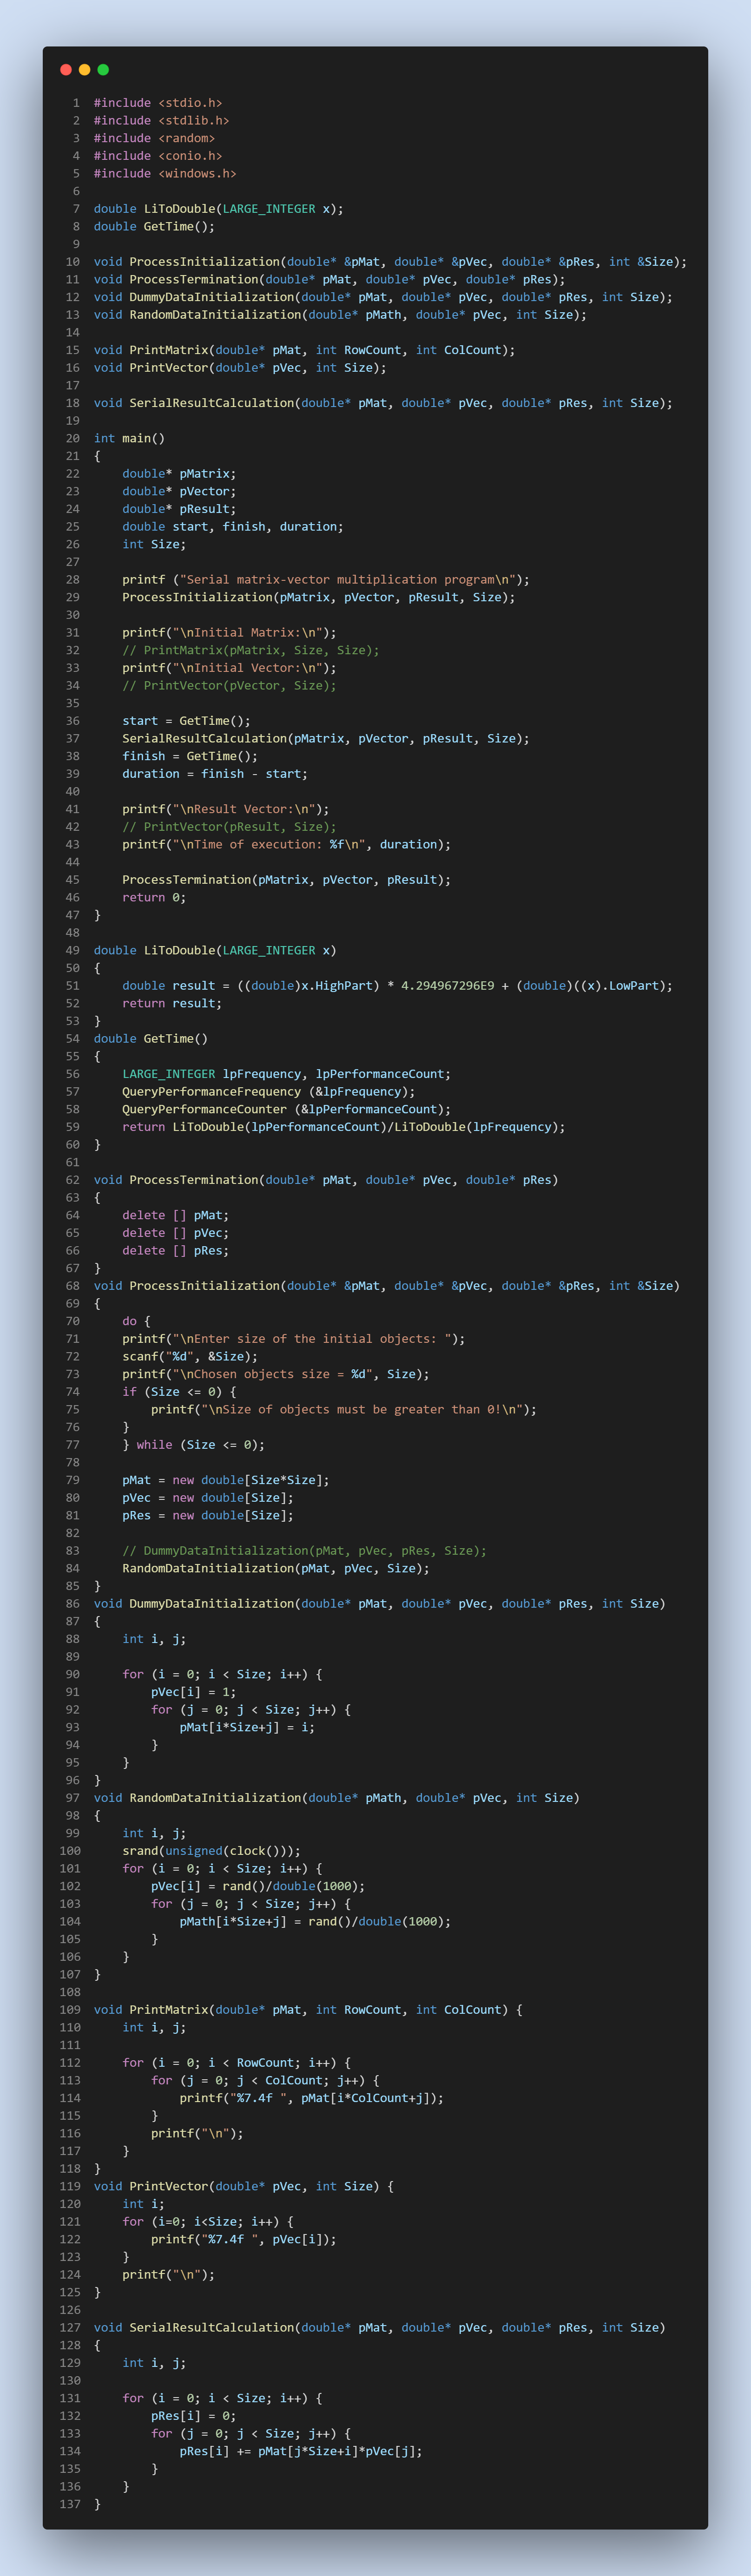
\includegraphics[trim=0in 52in 0in 0in, clip, scale=0.25]{./Photos/MatMul/serial.PNG}\clearpage
    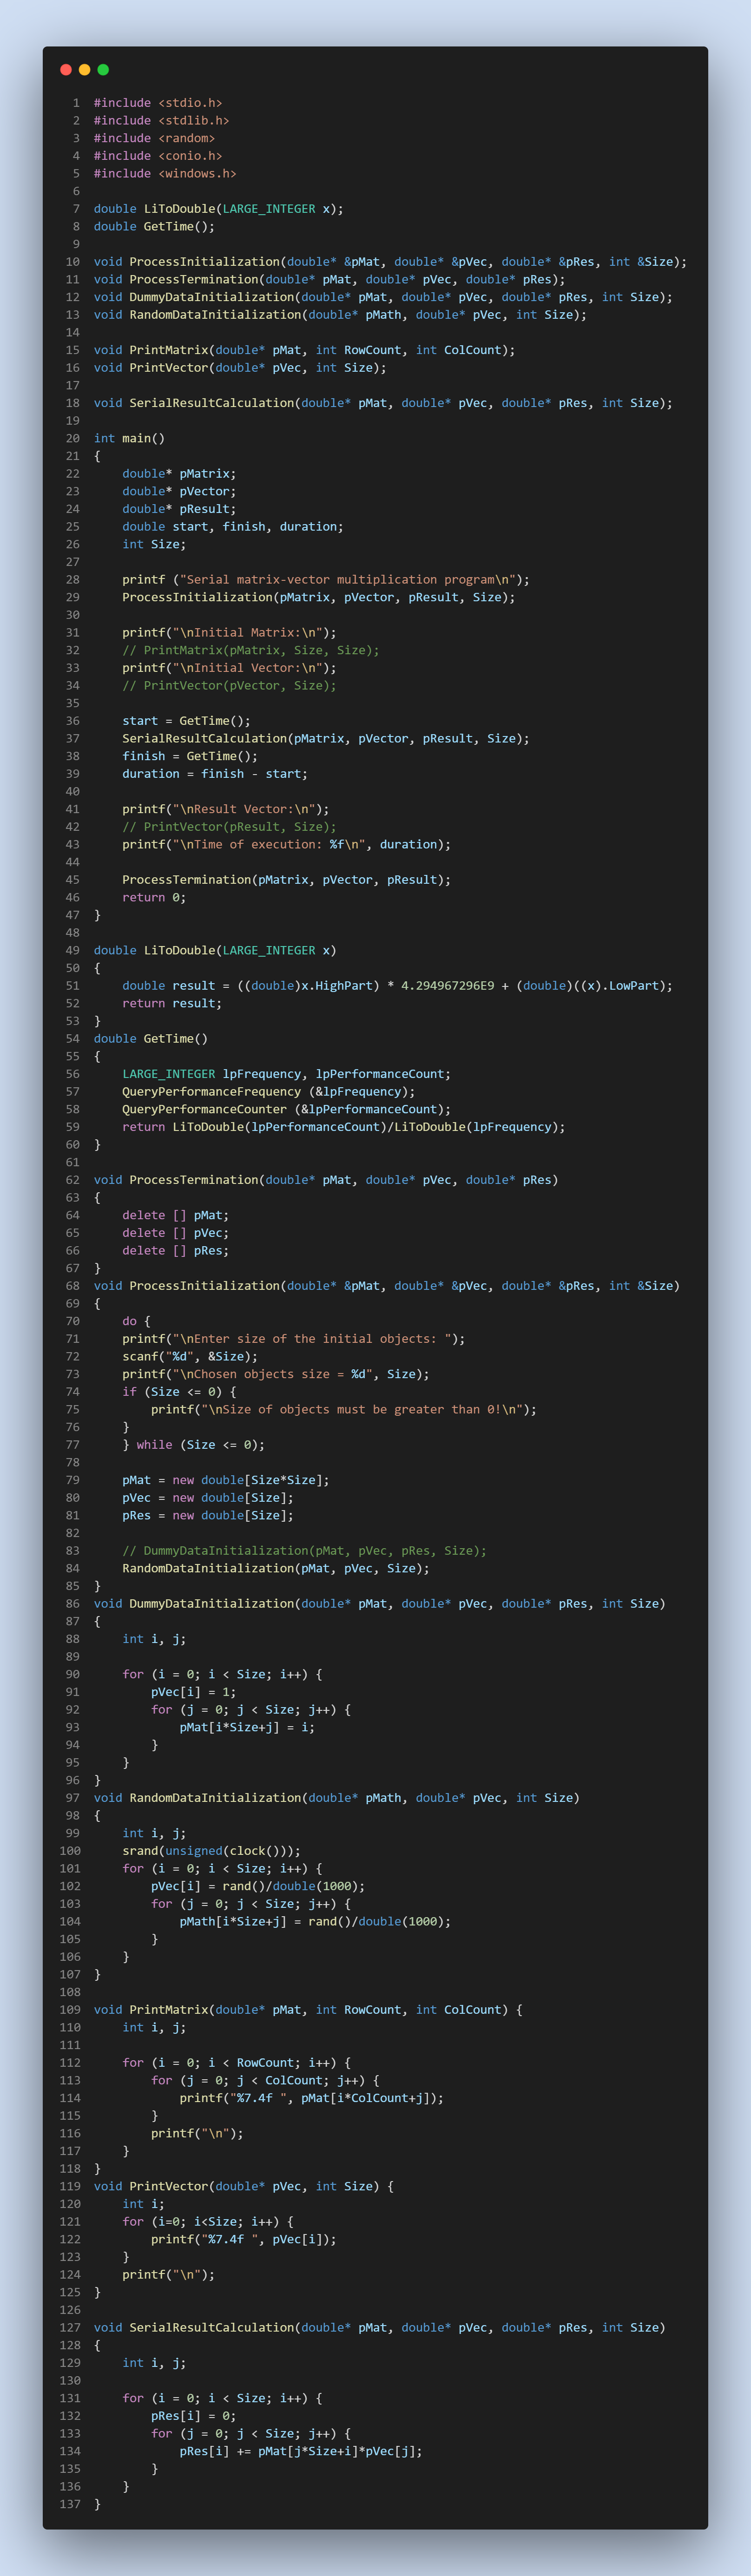
\includegraphics[trim=0in 16in 0in 25in, clip, scale=0.25]{./Photos/MatMul/serial.PNG}\clearpage
    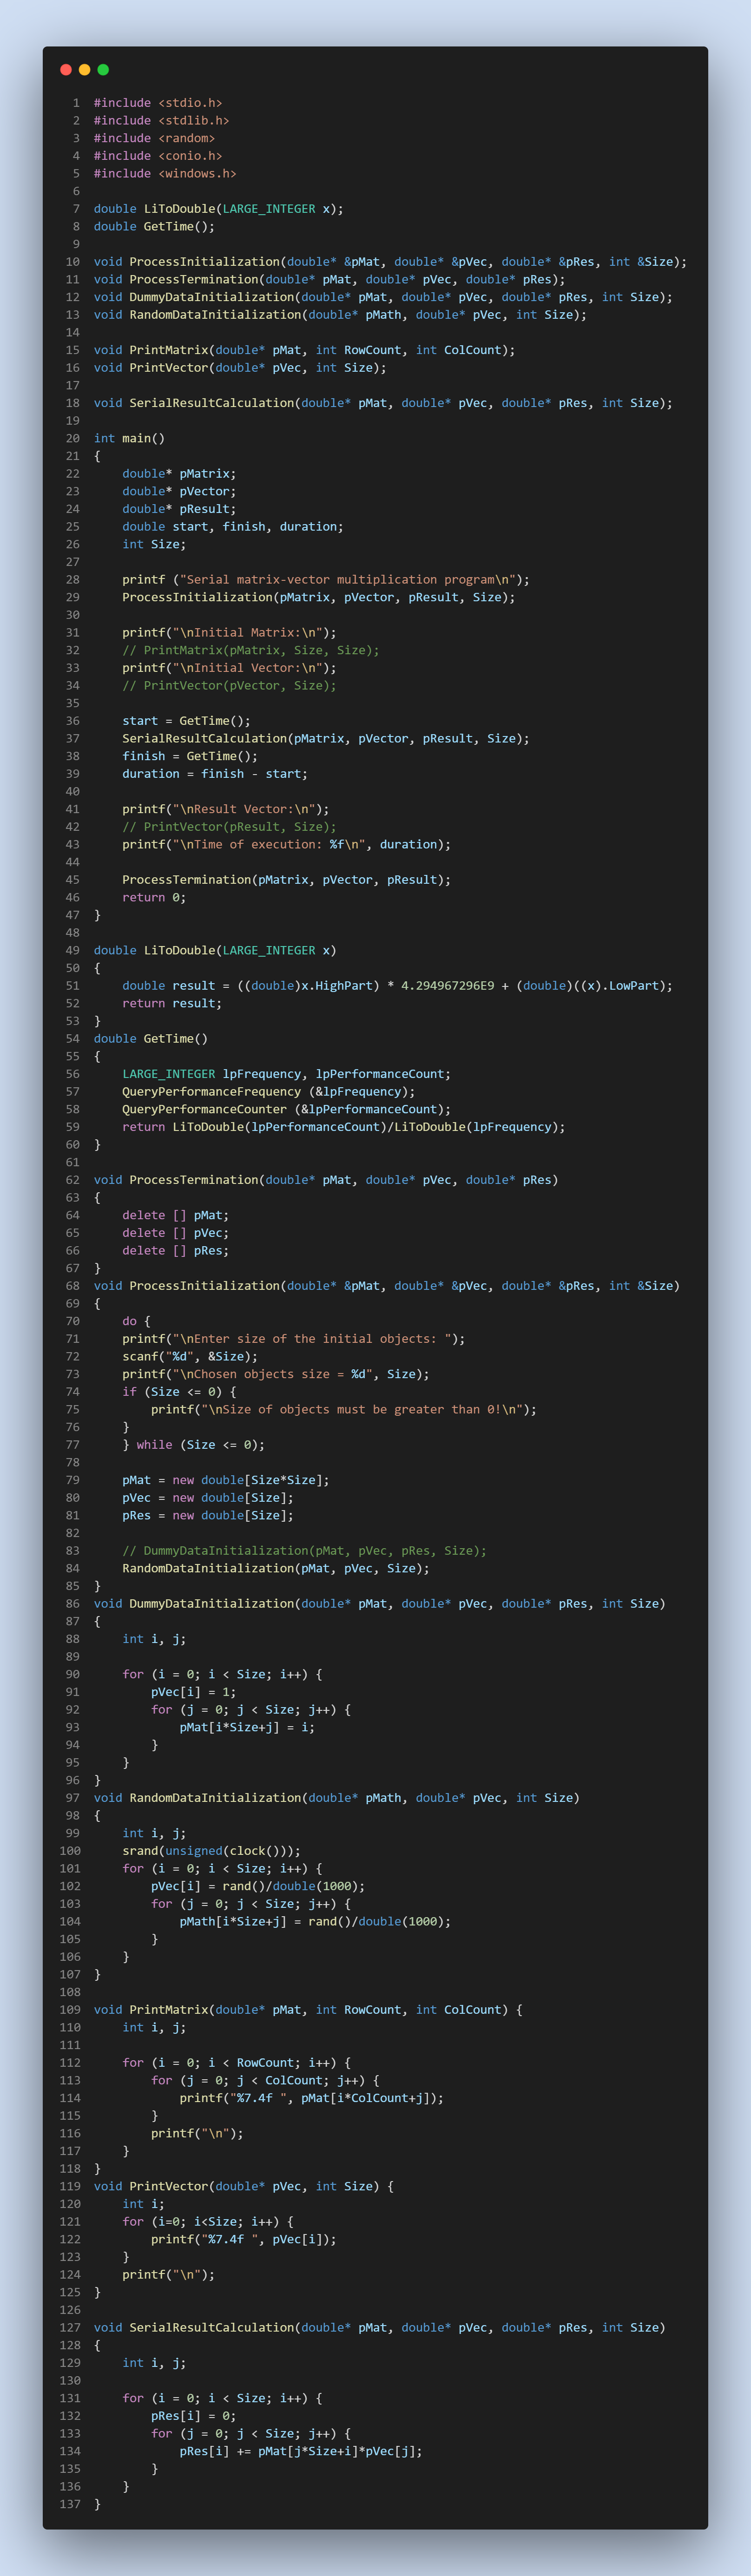
\includegraphics[trim=0in 0in 0in 61in, clip, scale=0.25]{./Photos/MatMul/serial.PNG}
\end{center}
\section{Thuật toán song song}
\begin{center}
	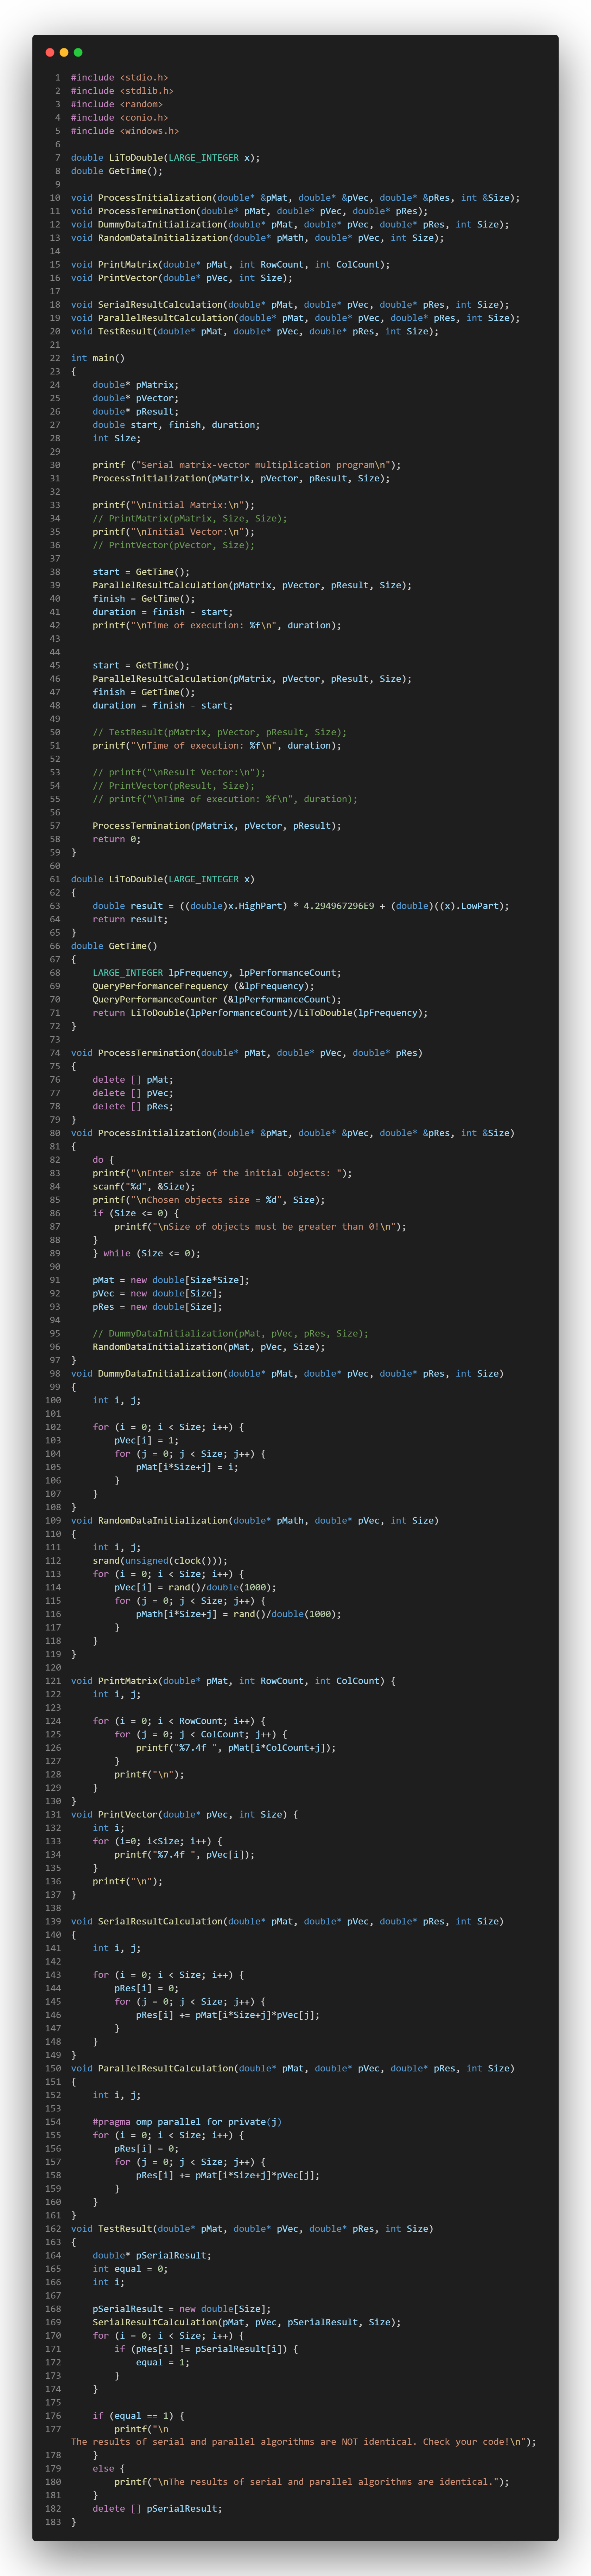
\includegraphics[trim=0in 85in 0in 0in, clip, scale=0.25]{./Photos/MatMul/parallel.PNG}
\clearpage
	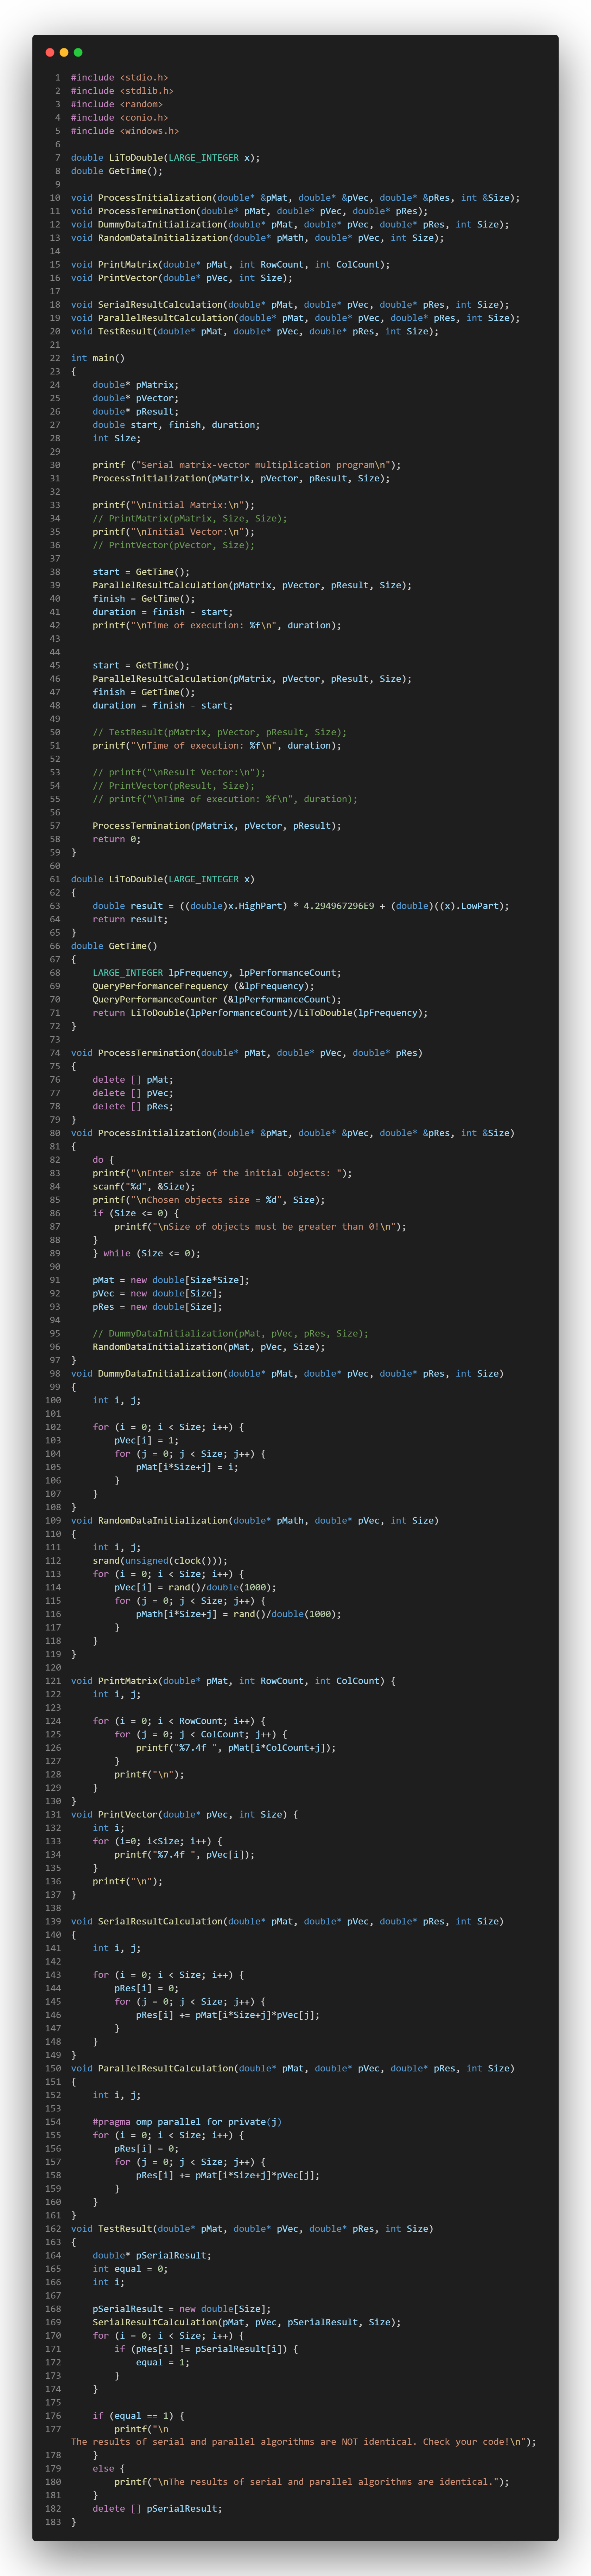
\includegraphics[trim=0in 49.5in 0in 16.5in, clip, scale=0.25]{./Photos/MatMul/parallel.PNG}
\clearpage
	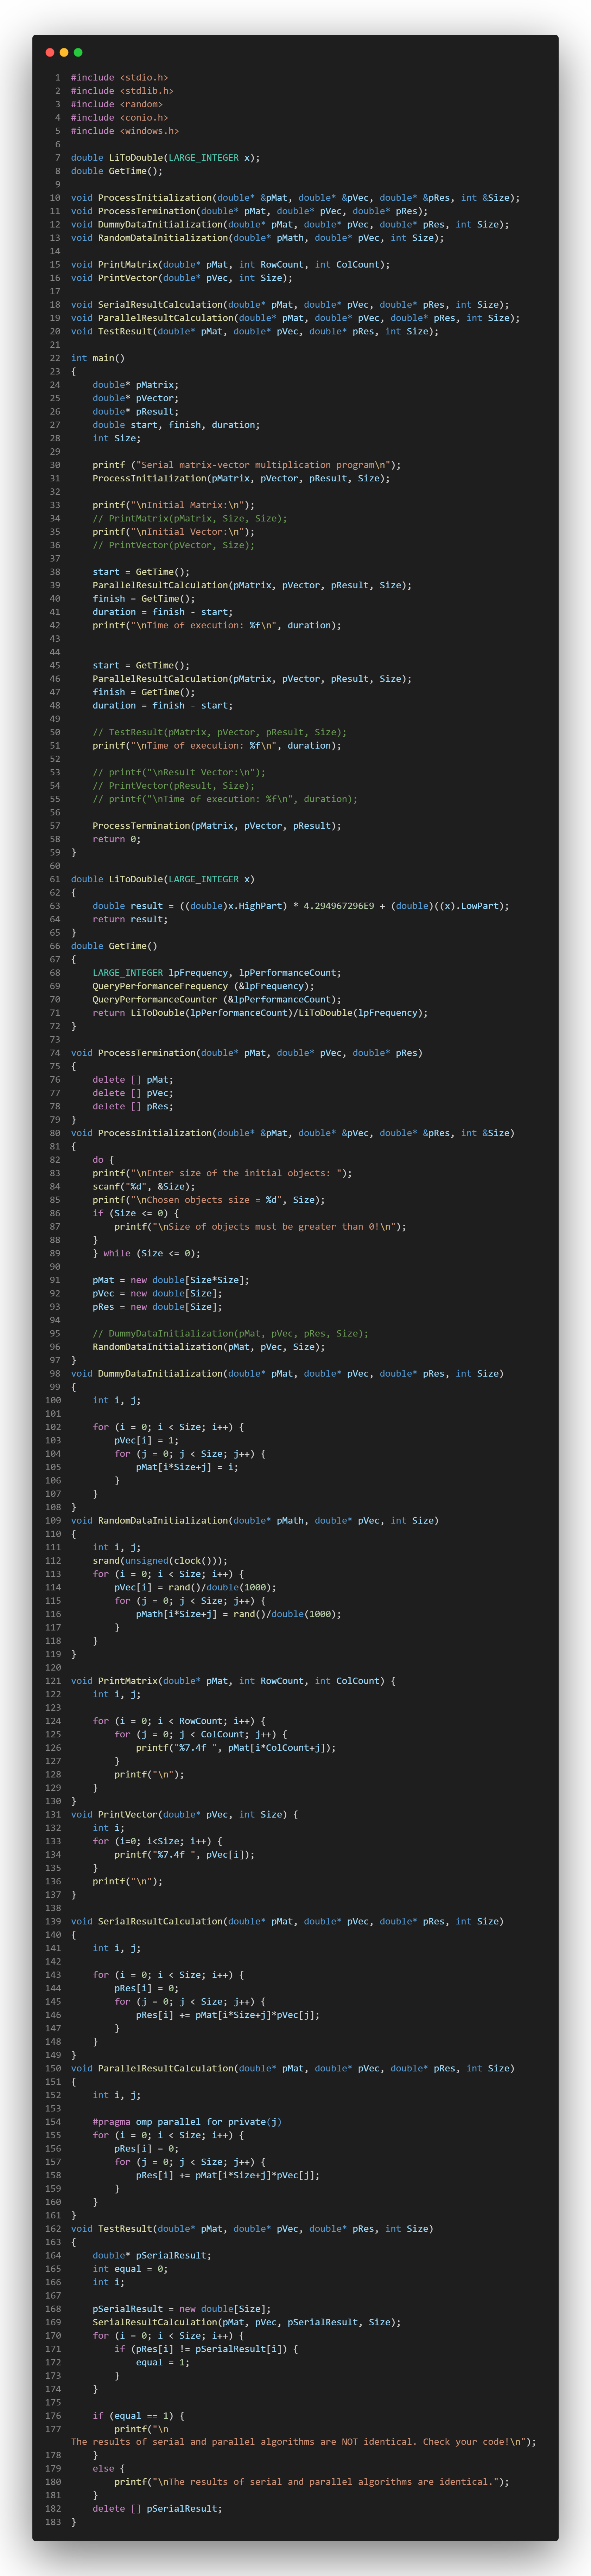
\includegraphics[trim=0in 15in 0in 52in, clip, scale=0.25]{./Photos/MatMul/parallel.PNG}
\clearpage
	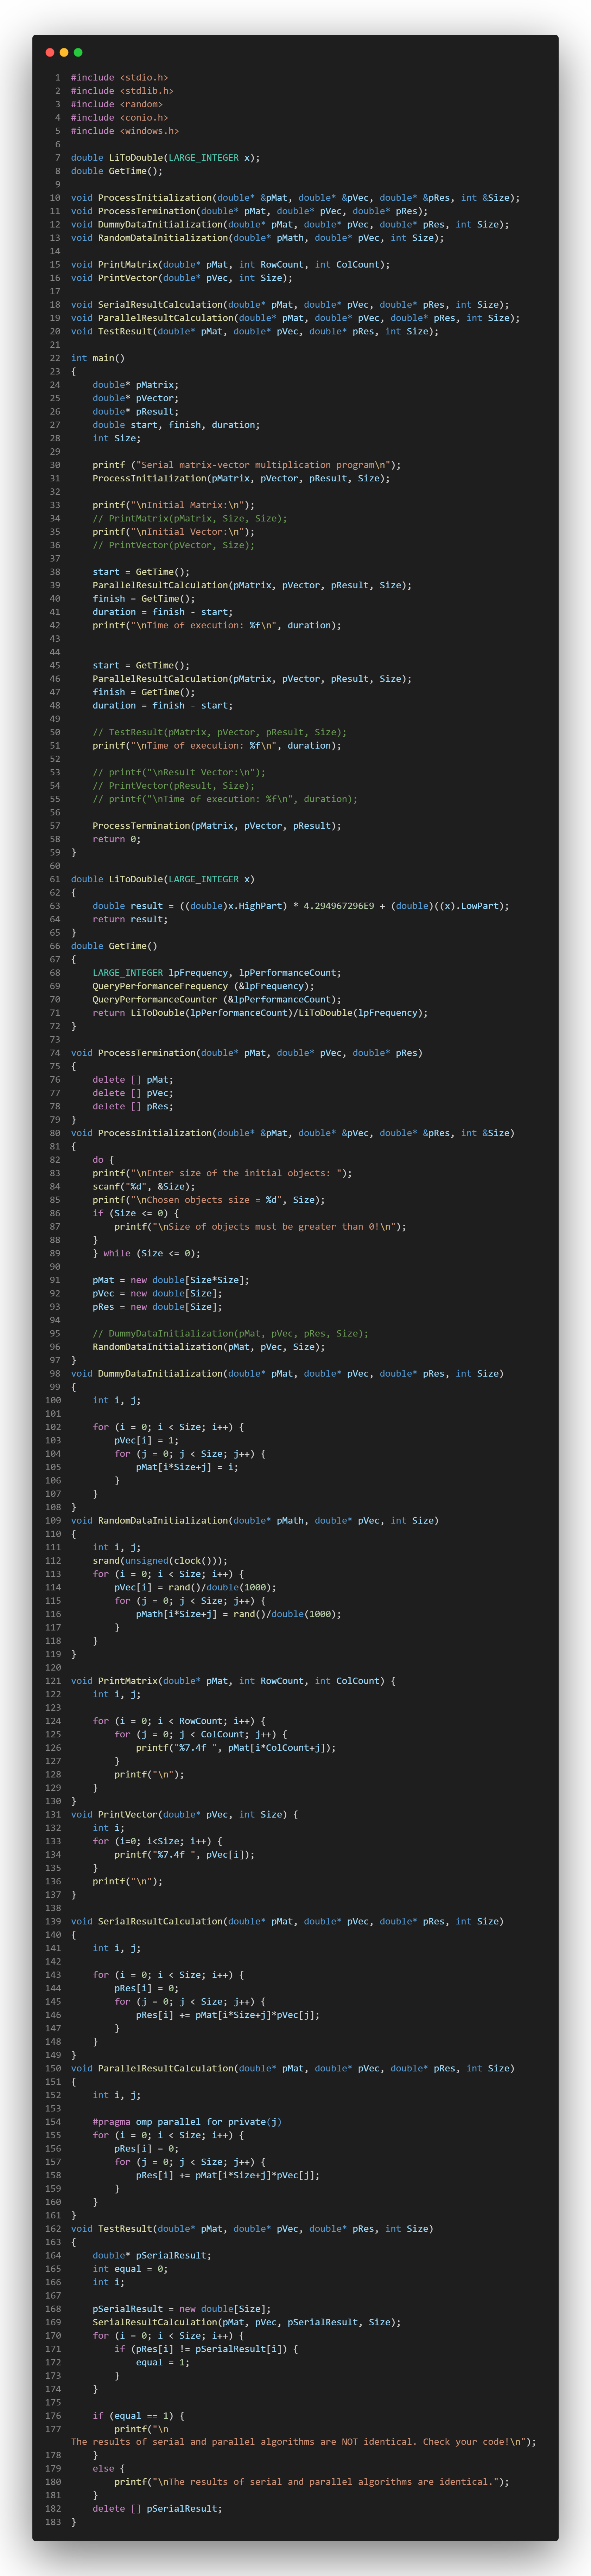
\includegraphics[trim=0in 0in 0in 86.5in, clip, scale=0.25]{./Photos/MatMul/parallel.PNG}
\end{center}
\section{Đánh giá}
\begin{center}
	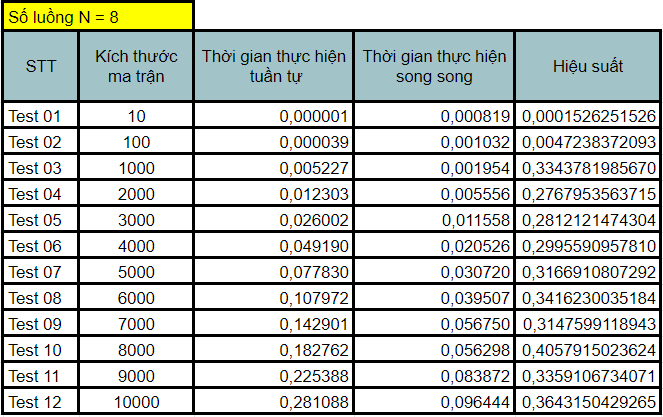
\includegraphics[scale=0.9]{./Photos/MatMul/Benchmark.PNG}
\end{center}

\chapter{Tìm số nguyên tố}
\section{Thuật toán tuần tự}
\begin{center}
	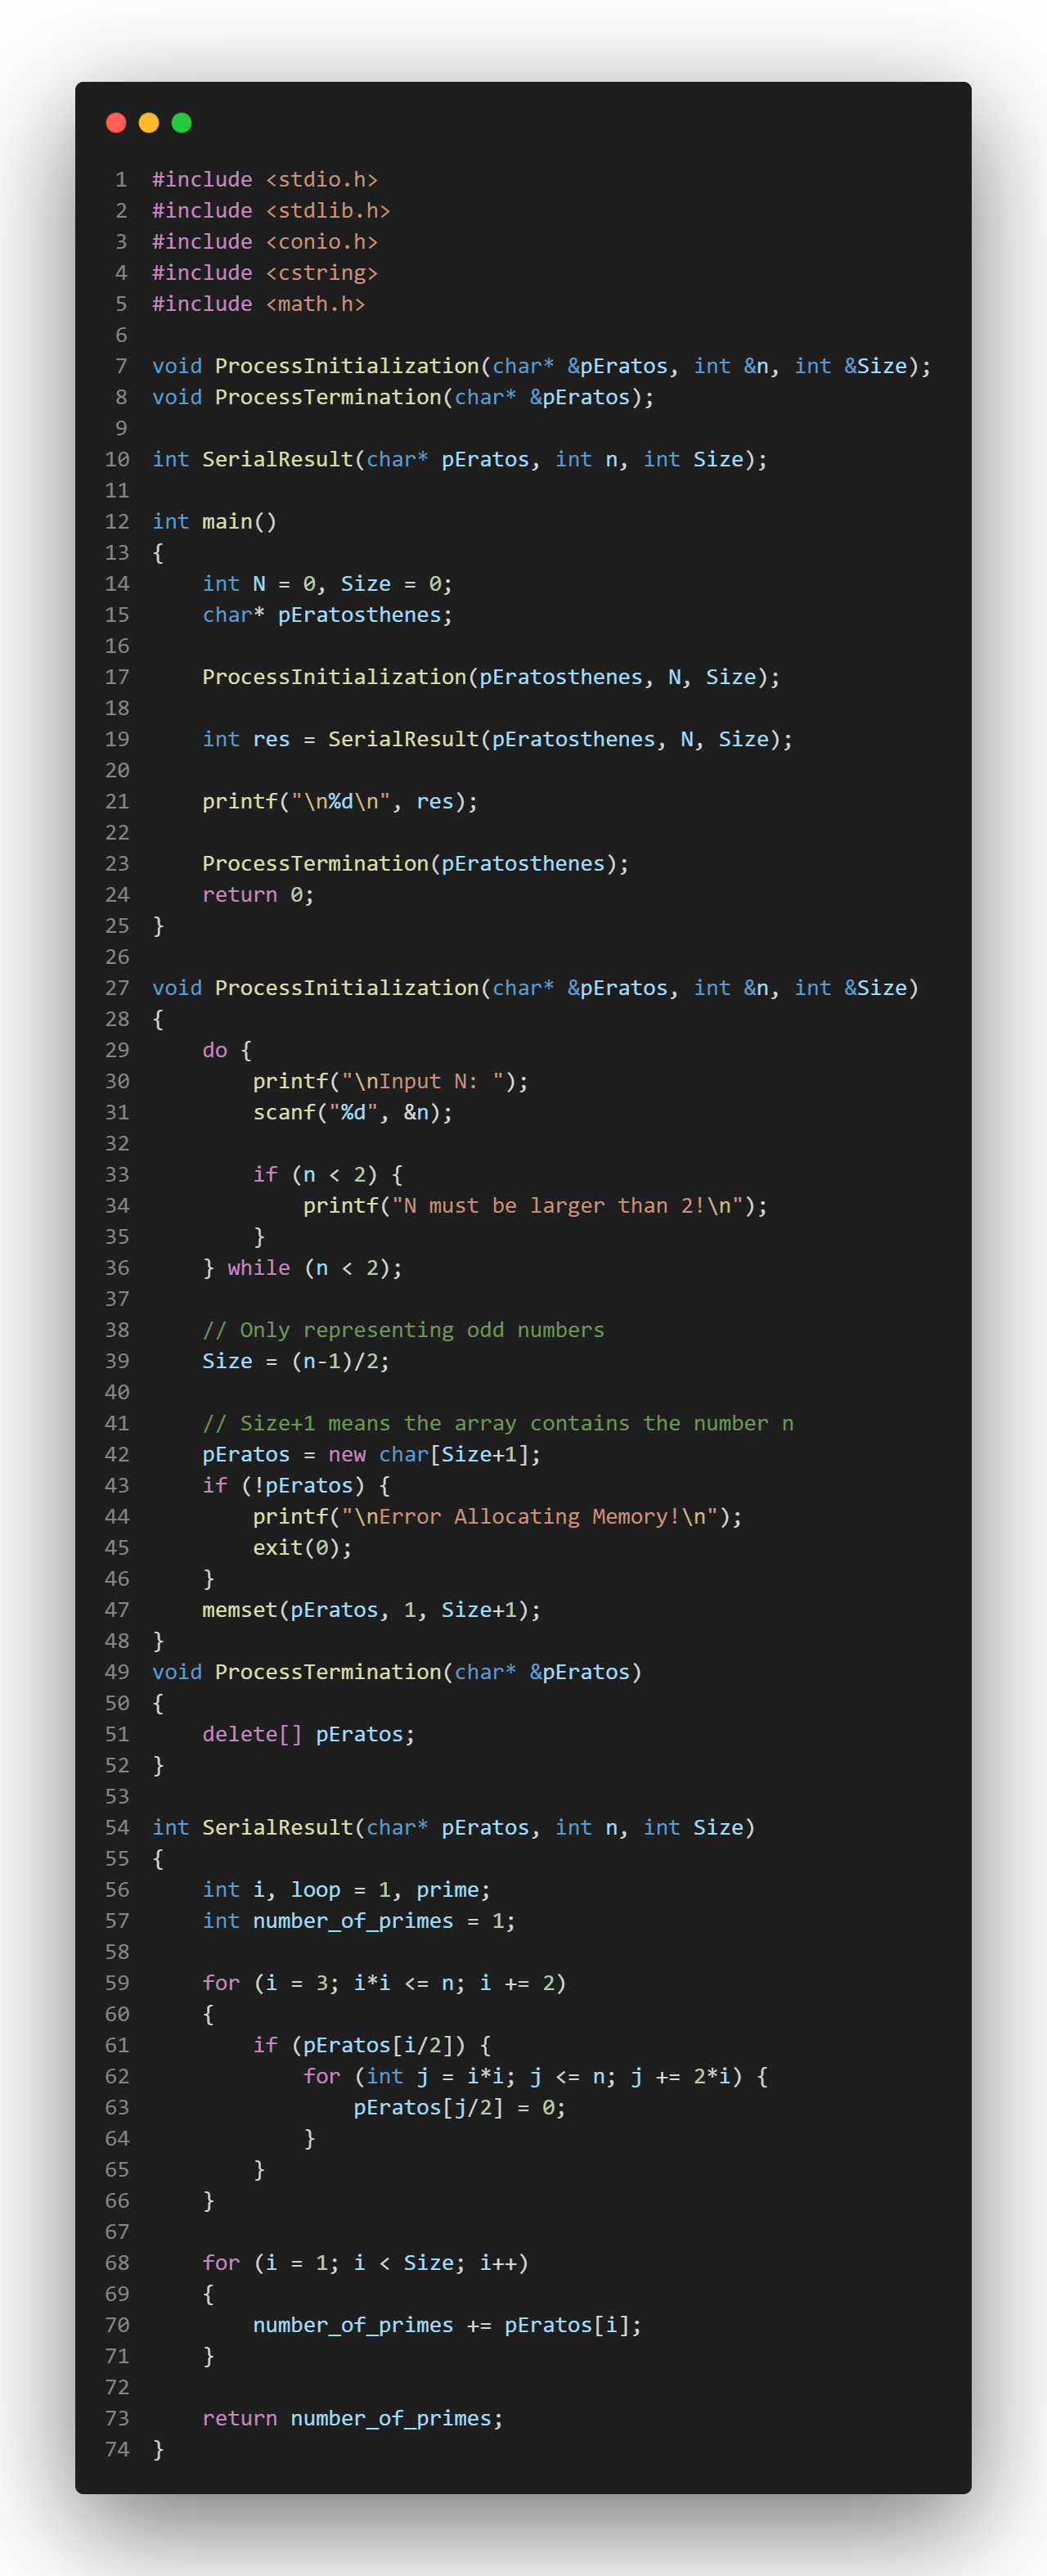
\includegraphics[trim=0in 27in 0in 0in, clip, scale=0.35]{./Photos/Primes/Serial.PNG}
\clearpage
	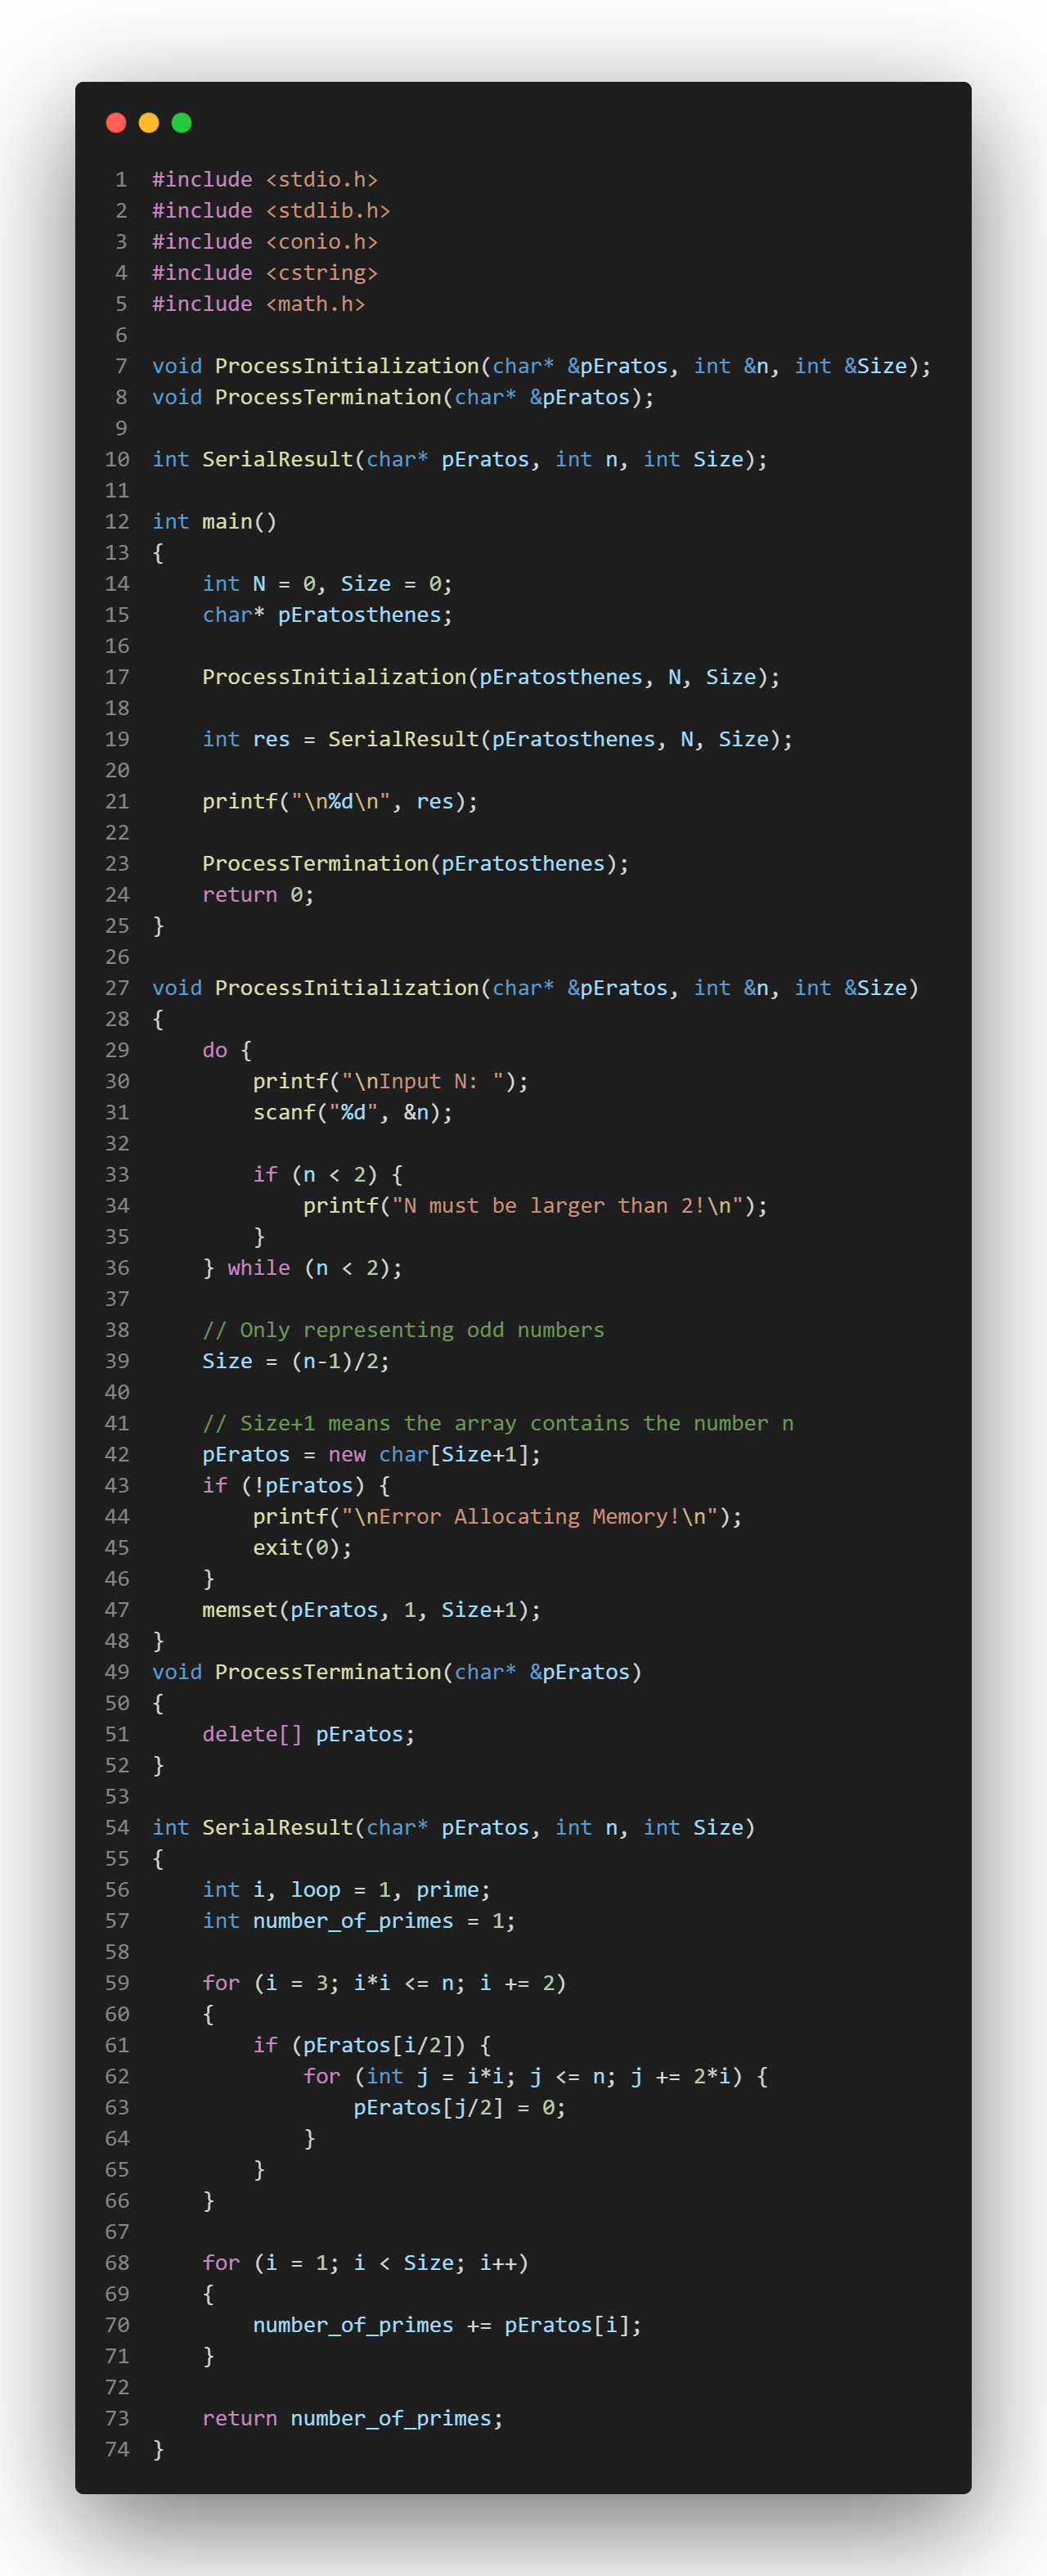
\includegraphics[trim=0in 1.5in 0in 16.5in, clip, scale=0.35]{./Photos/Primes/Serial.PNG}
\end{center}
\section{Thuật toán song song}
\begin{center}
	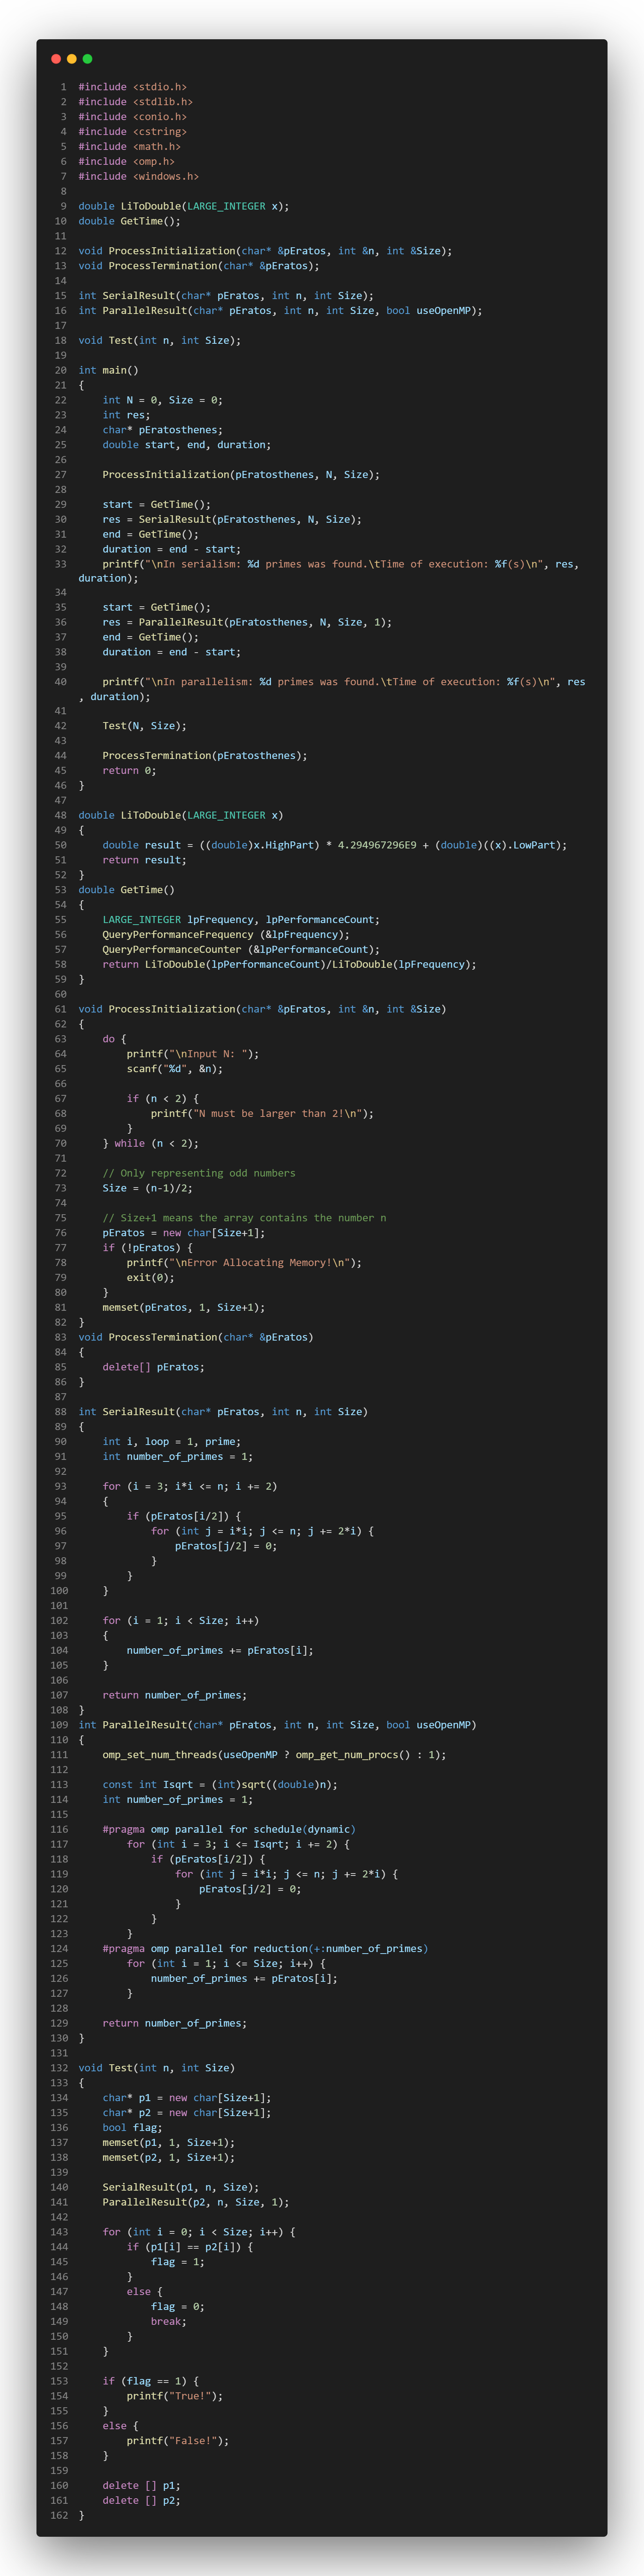
\includegraphics[trim=0in 57.75in 0in 0in, clip, scale=0.25]{./Photos/Primes/Parallel.PNG}
\clearpage
	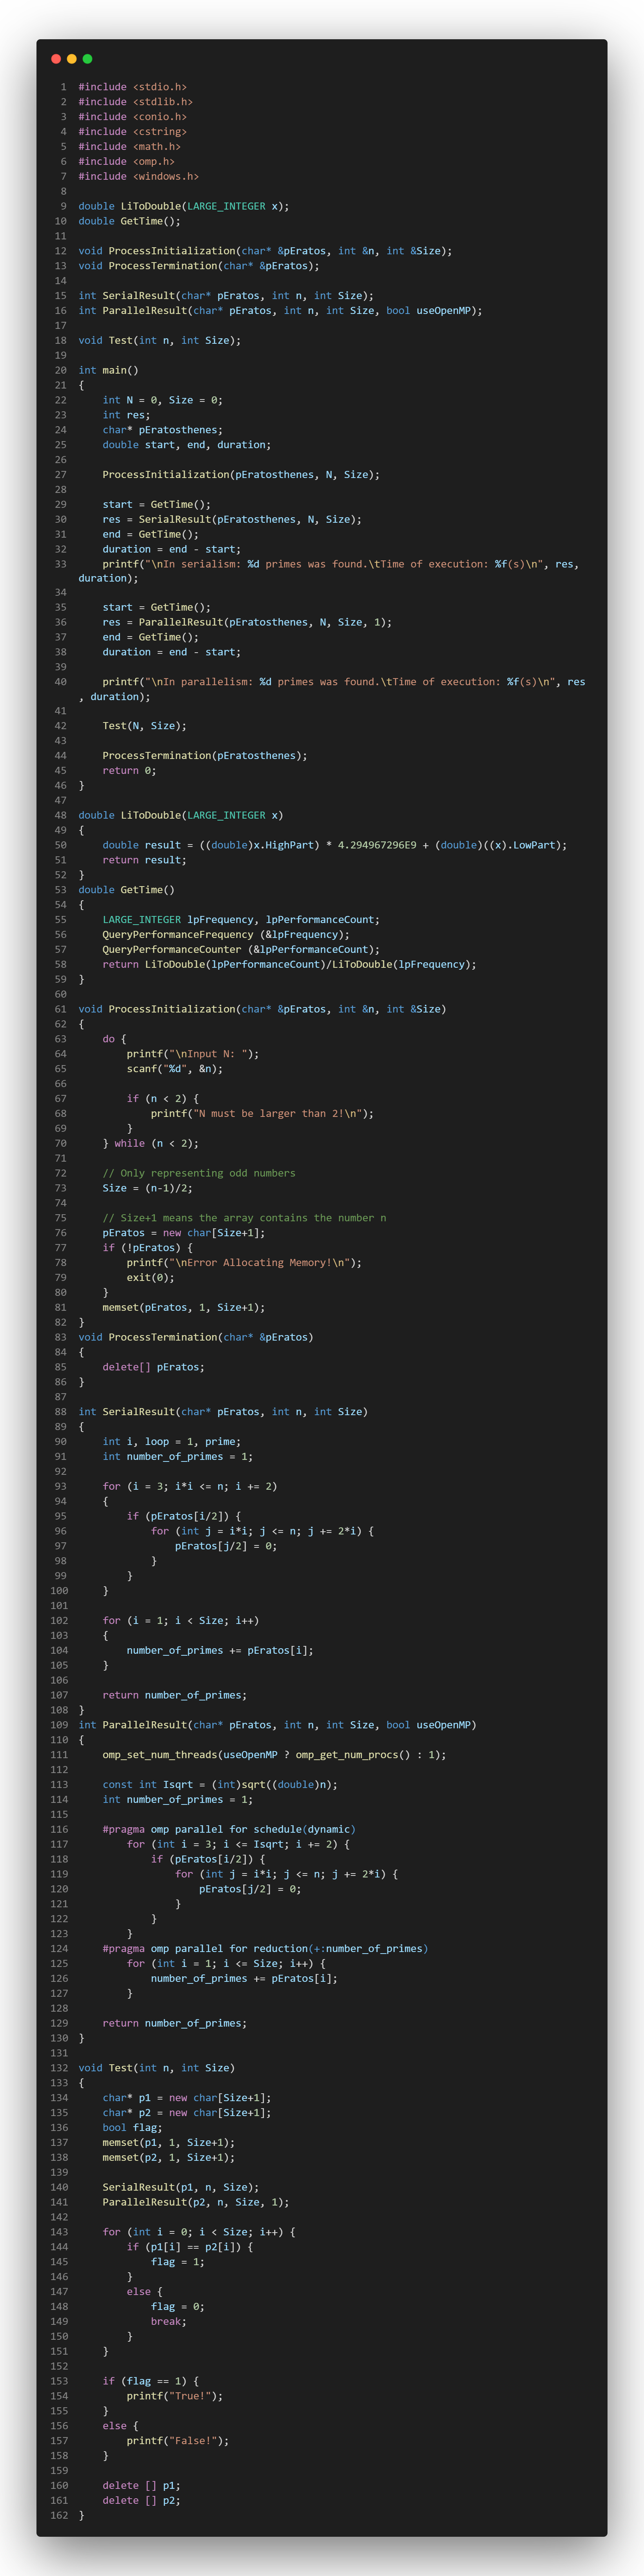
\includegraphics[trim=0in 22.3in 0in 33.25in, clip, scale=0.25]{./Photos/Primes/Parallel.PNG}
\clearpage
	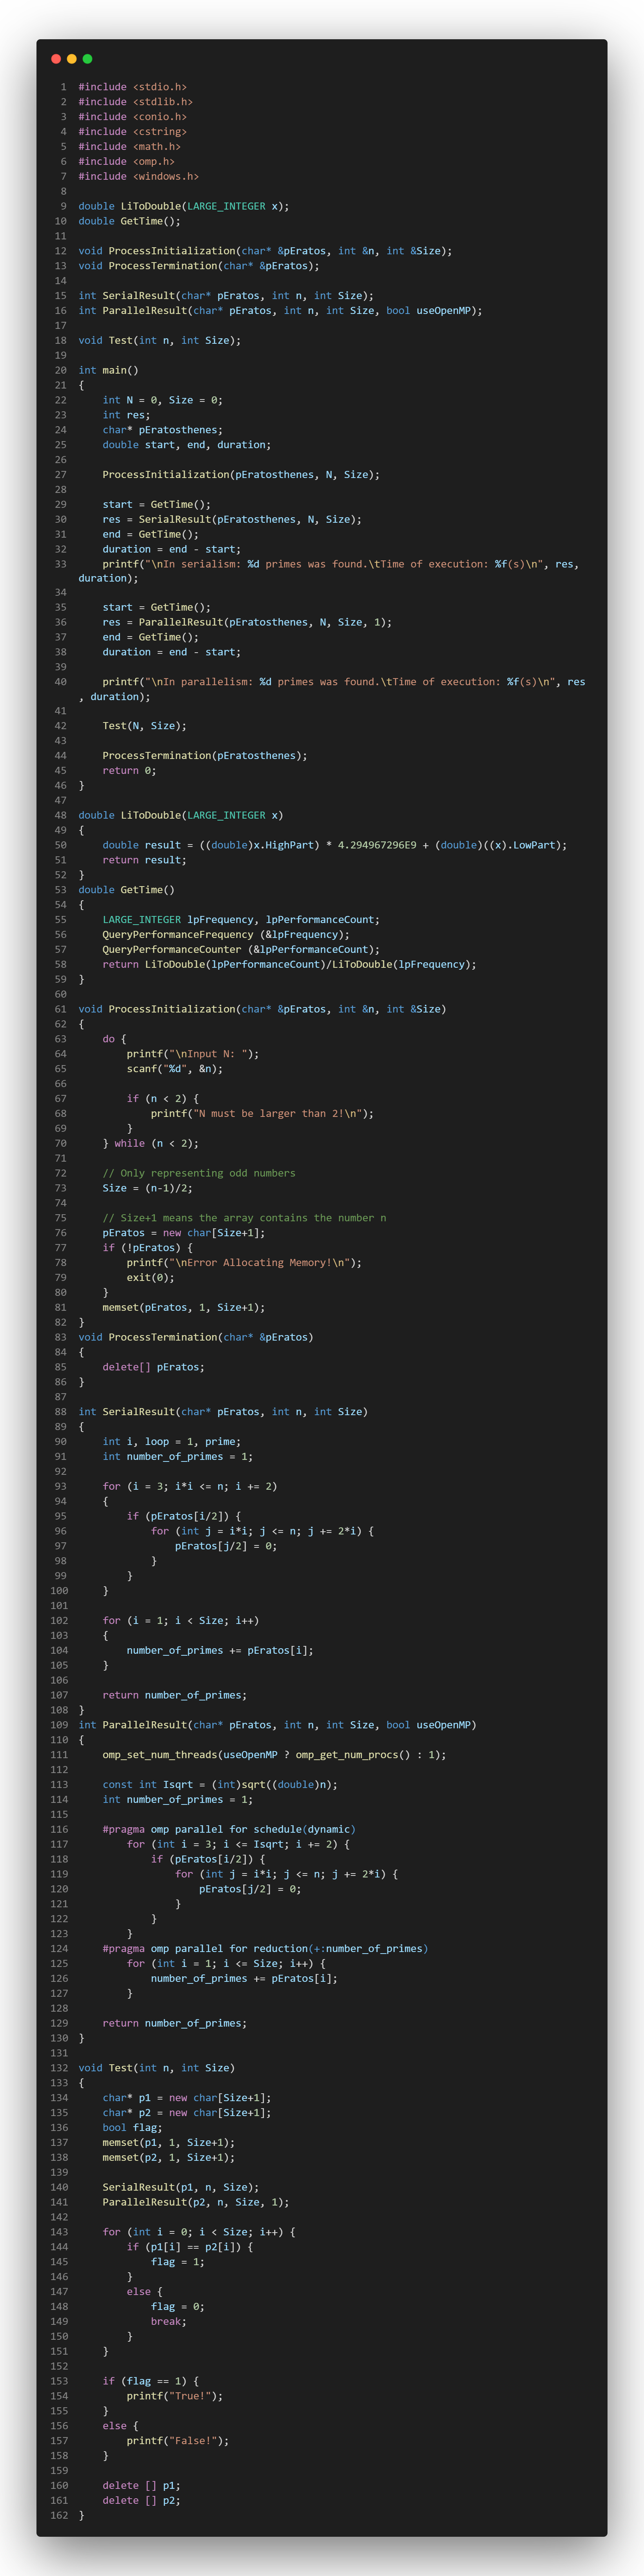
\includegraphics[trim=0in 0in 0in 68.55in, clip, scale=0.25]{./Photos/Primes/Parallel.PNG}
\end{center}
\section{Đánh giá}
\begin{center}
	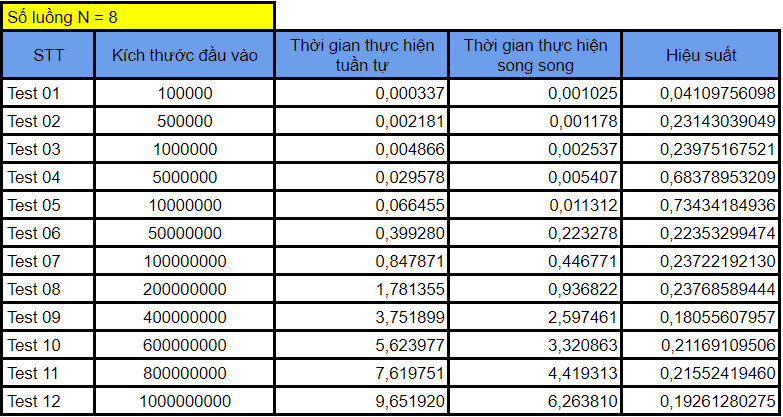
\includegraphics[scale=0.9]{./Photos/Primes/Benchmark.PNG}
\end{center}

\chapter{Tính số Fibonacci}
\section{Thuật toán tuần tự}
\begin{center}
	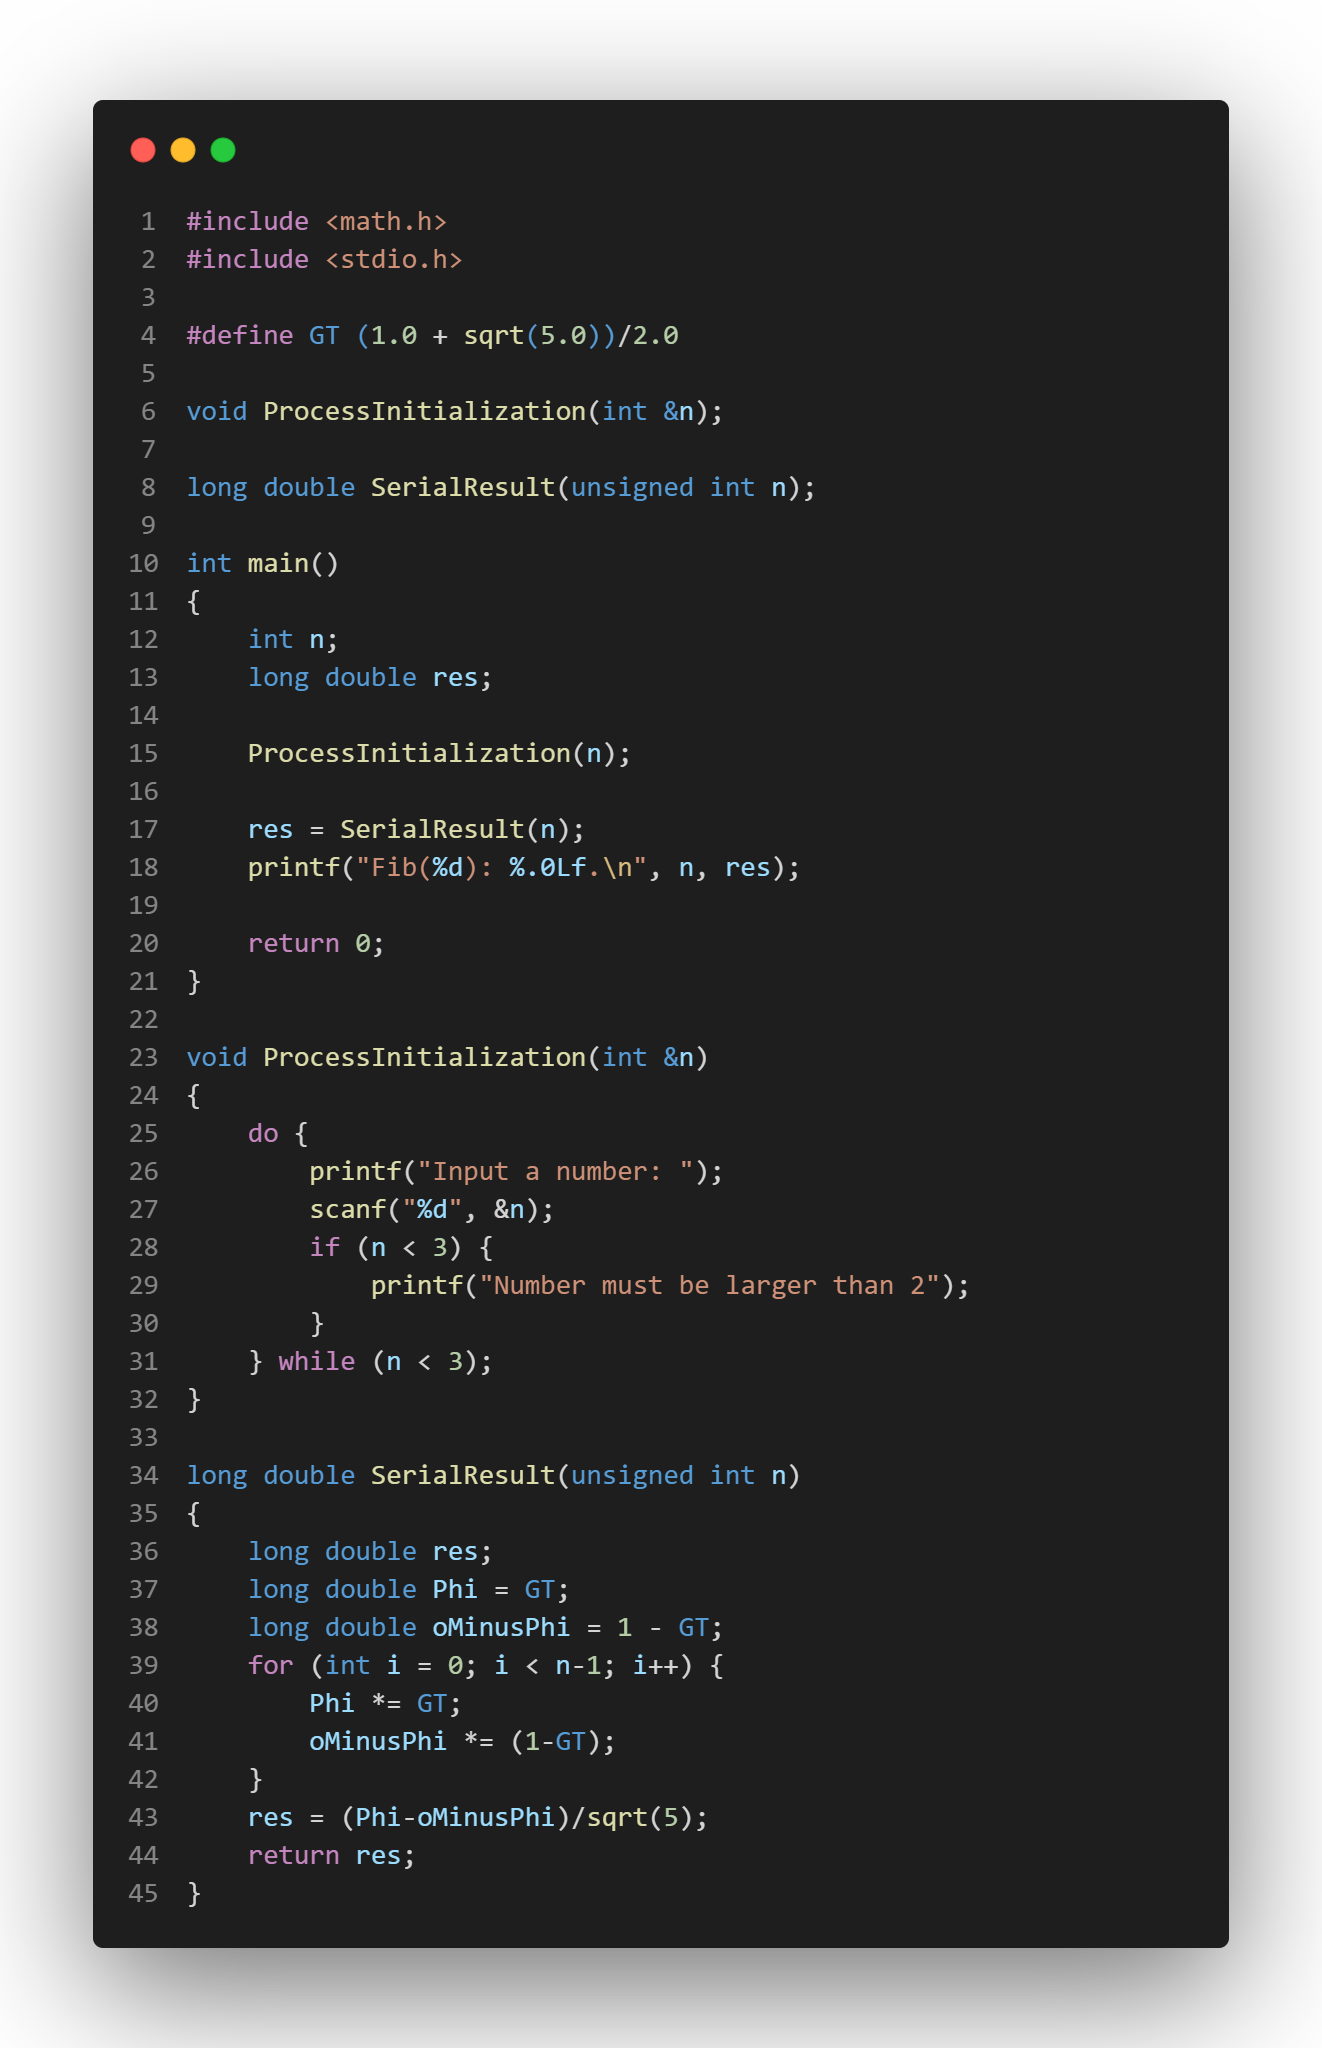
\includegraphics[trim=0in 12in 0in 0in, clip, scale=0.35]{./Photos/Fibonacci/Serial.PNG}
\clearpage
	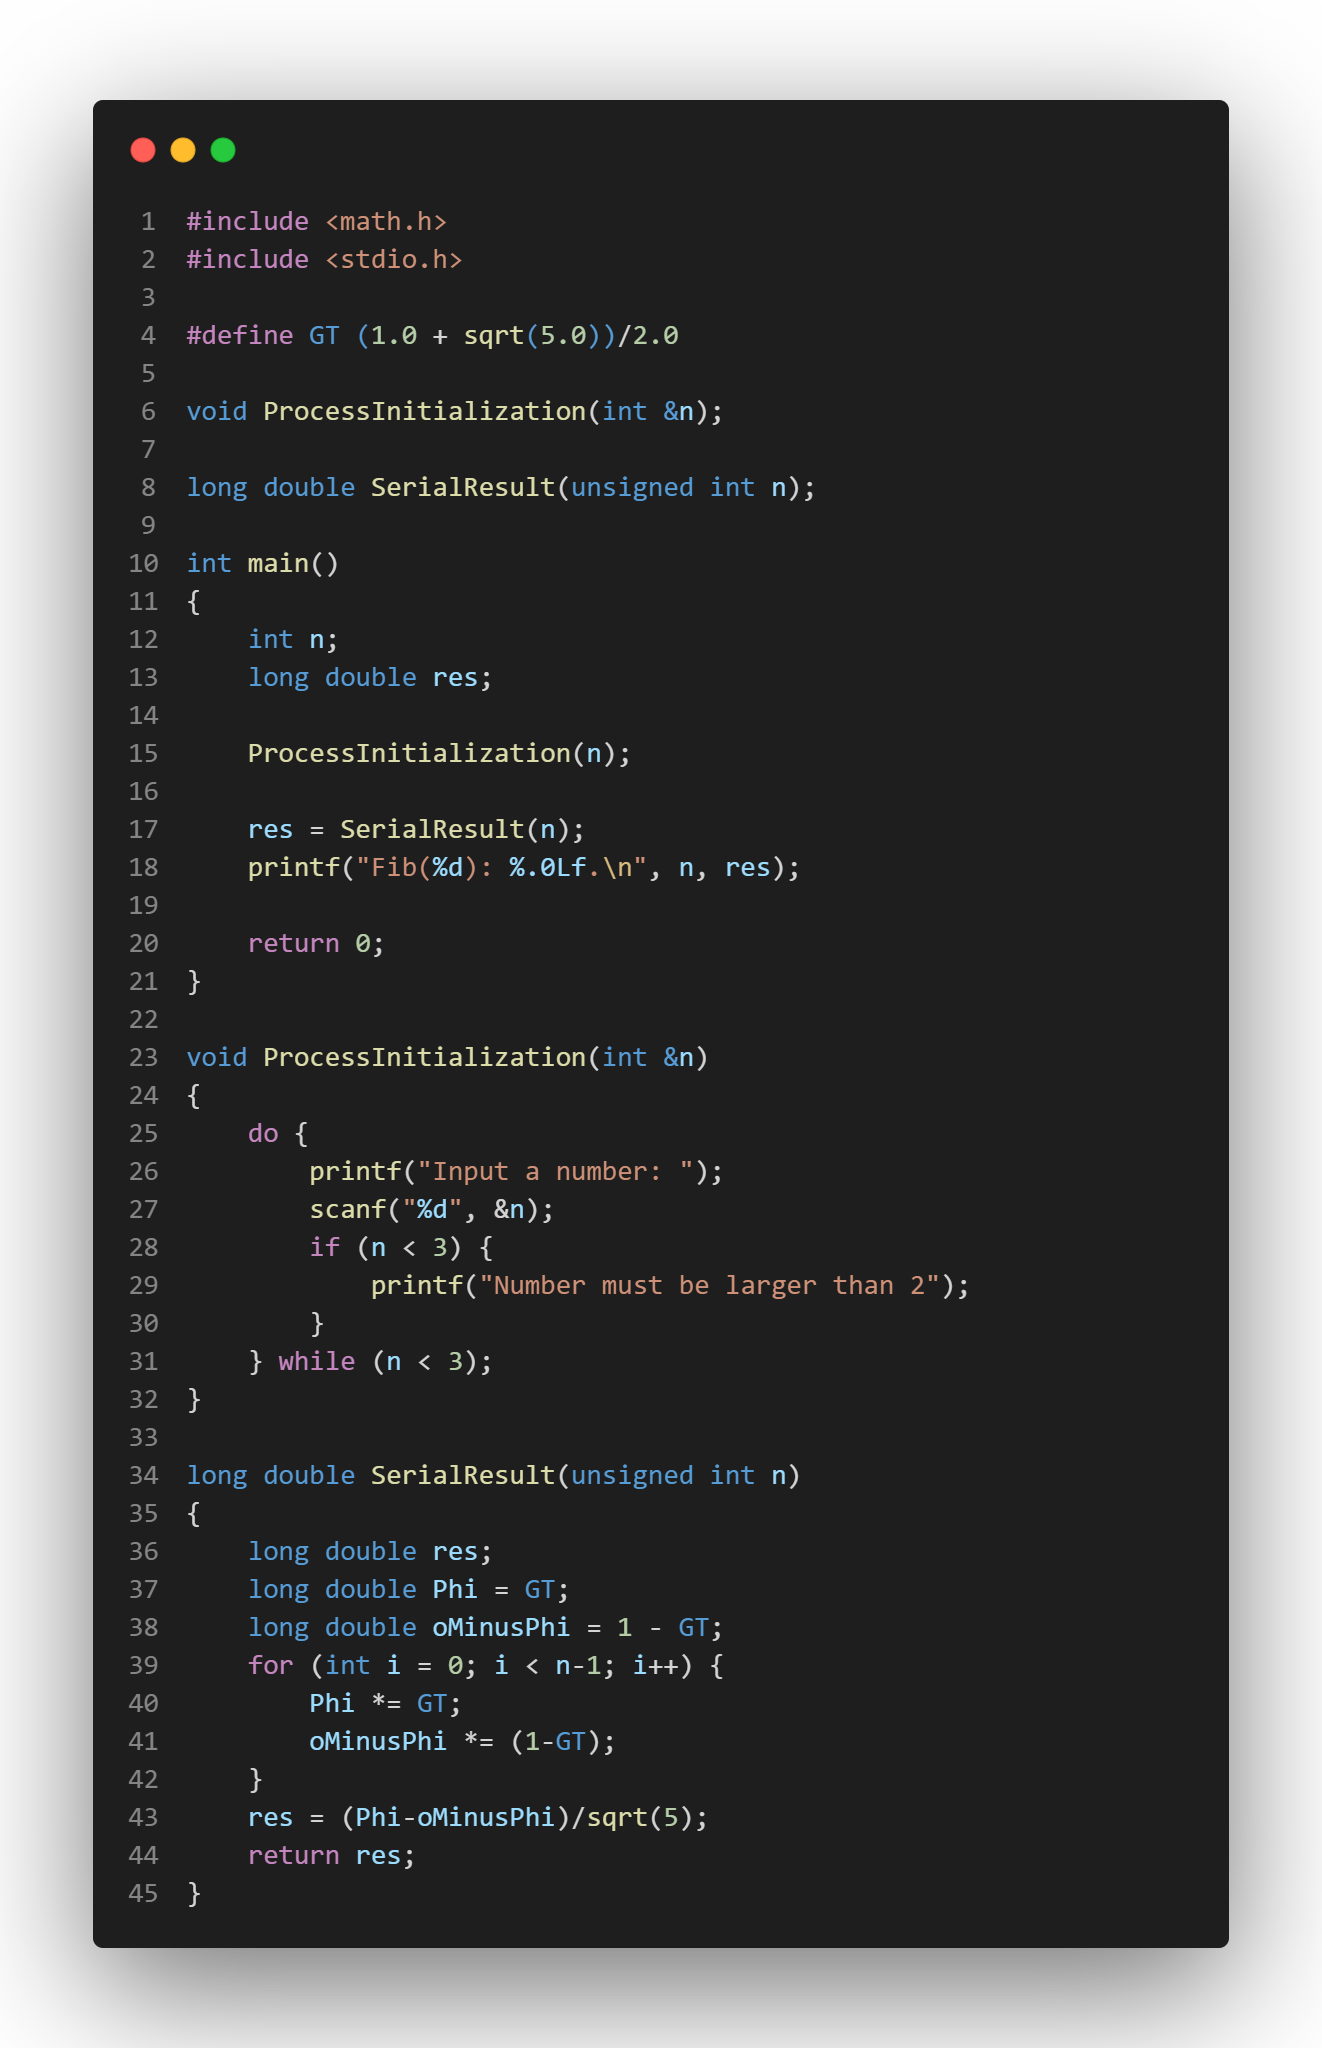
\includegraphics[trim=0in 0in 0in 16.5in, clip, scale=0.35]{./Photos/Fibonacci/Serial.PNG}
\end{center}
\section{Thuật toán song song}
\begin{center}
	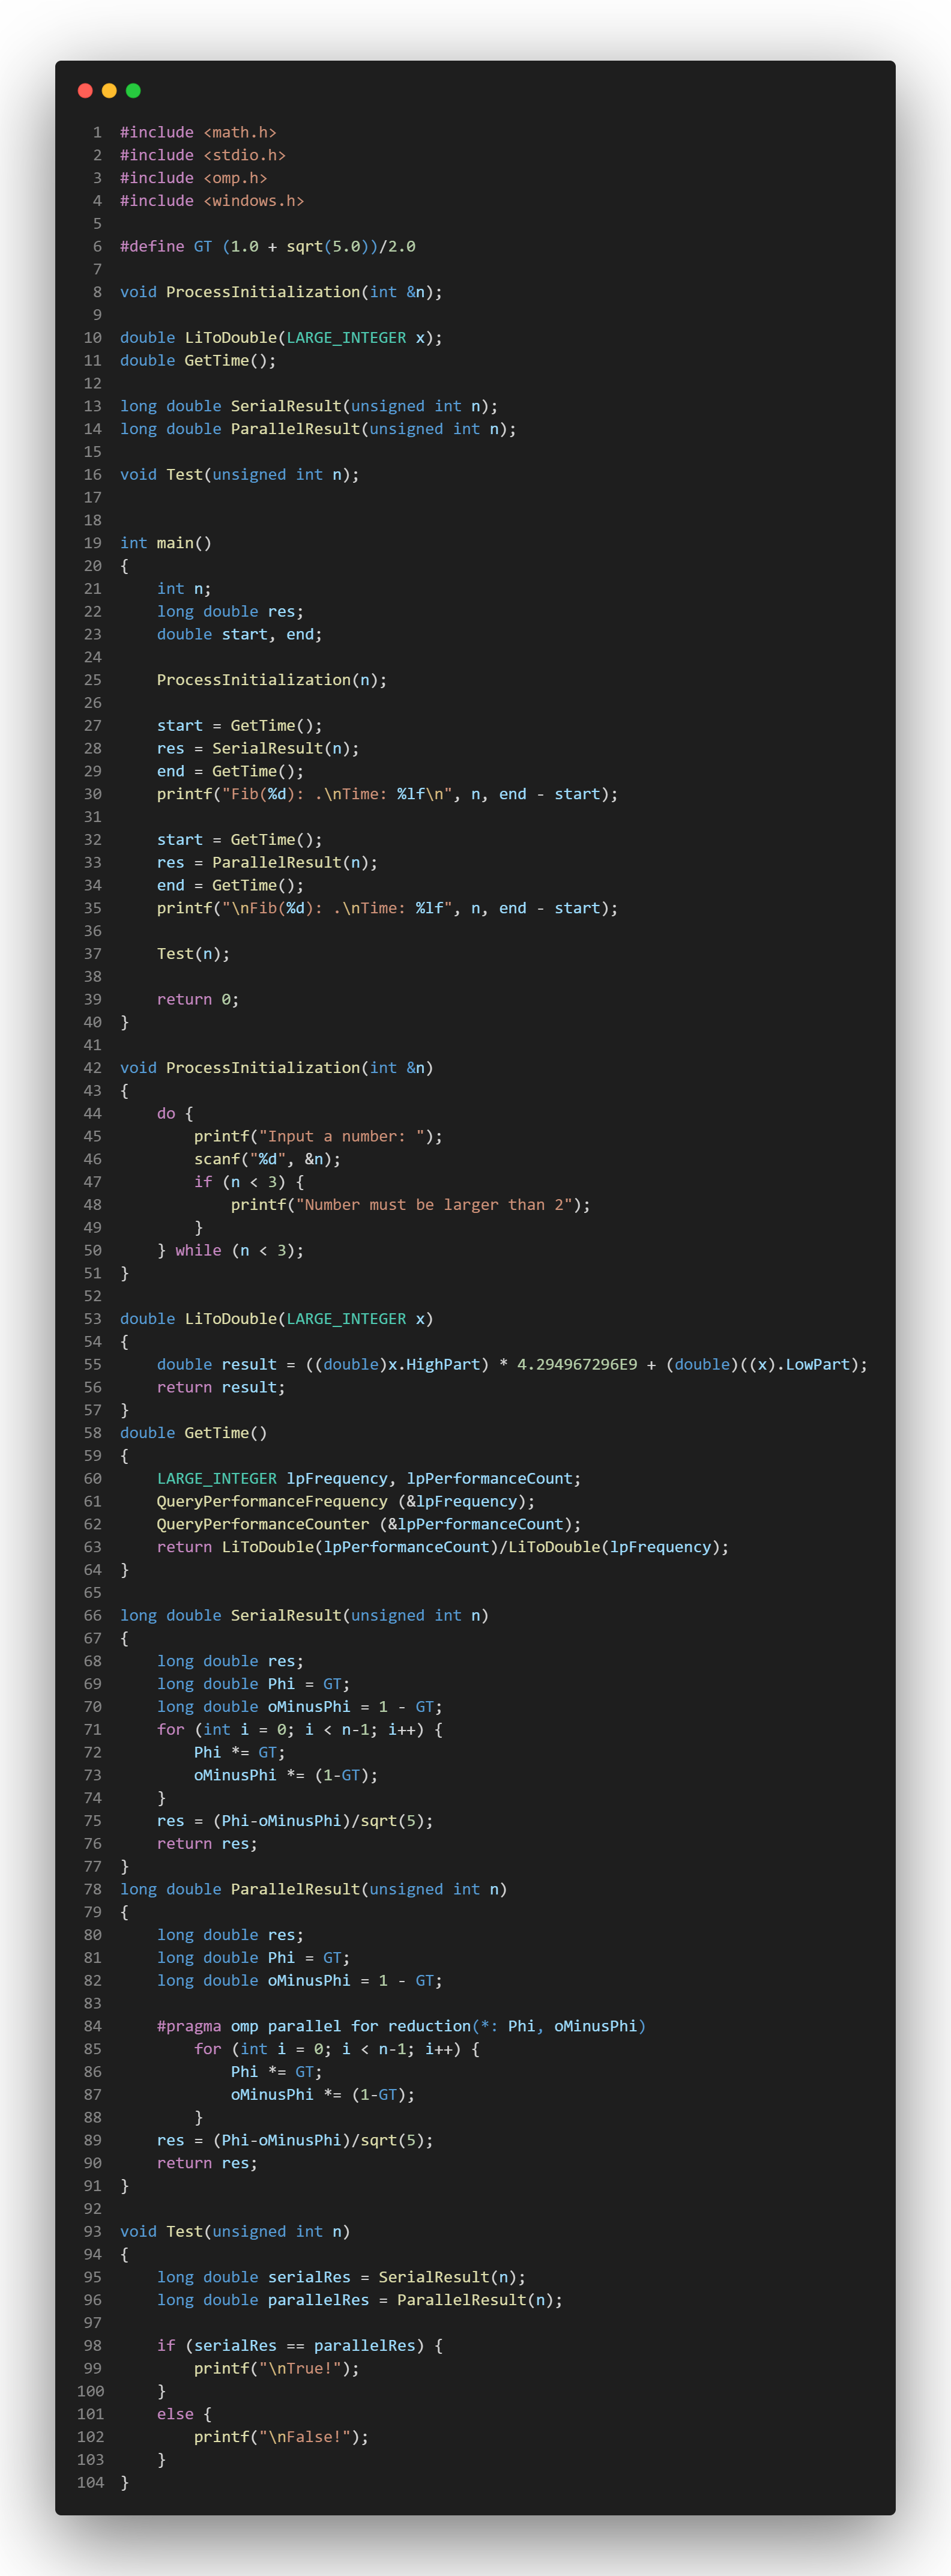
\includegraphics[trim=0in 45in 0in 0in, clip, scale=0.25]{./Photos/Fibonacci/Parallel.PNG}
\clearpage
	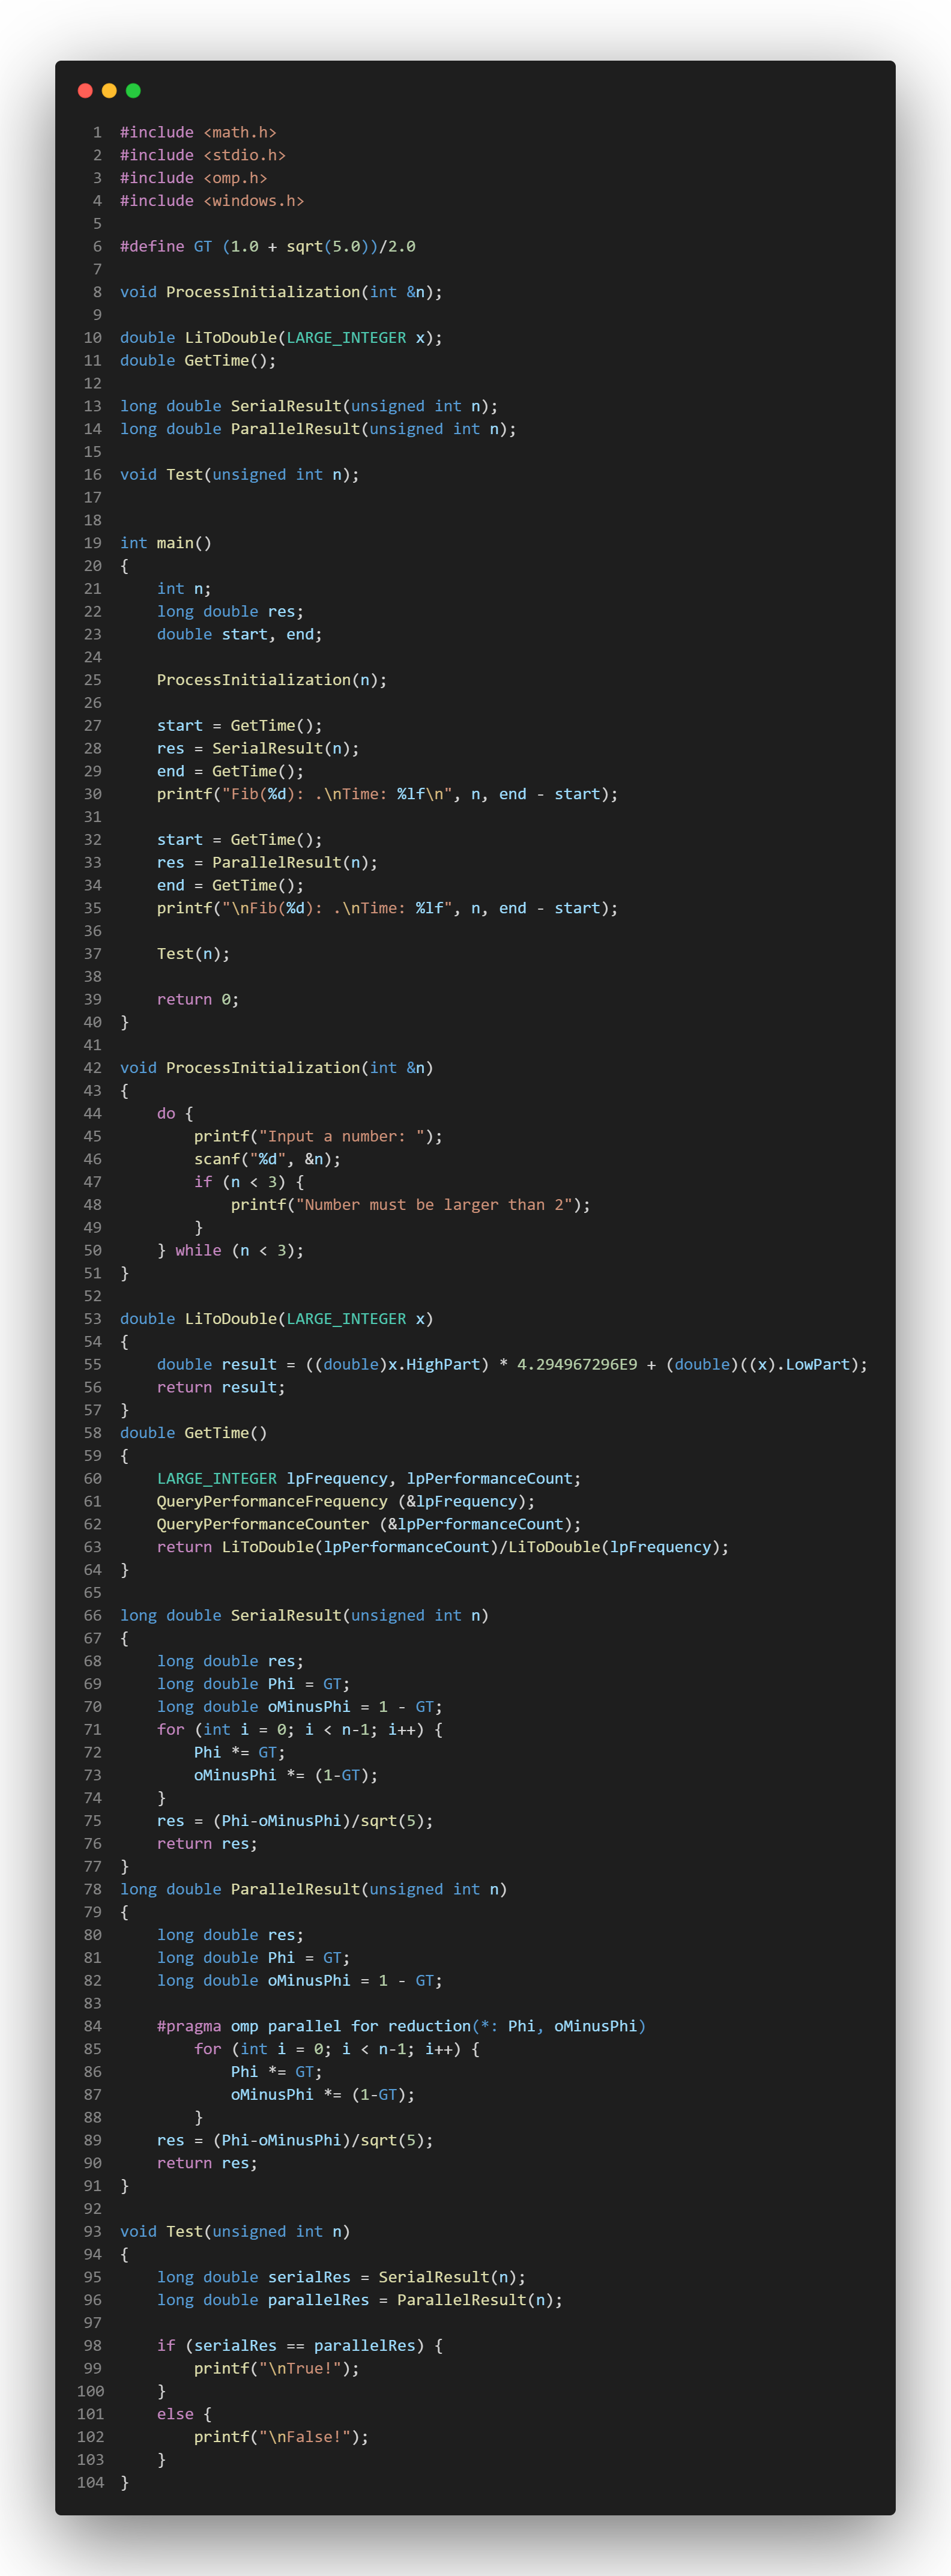
\includegraphics[trim=0in 9.75in 0in 14.25in, clip, scale=0.25]{./Photos/Fibonacci/Parallel.PNG}
\clearpage
	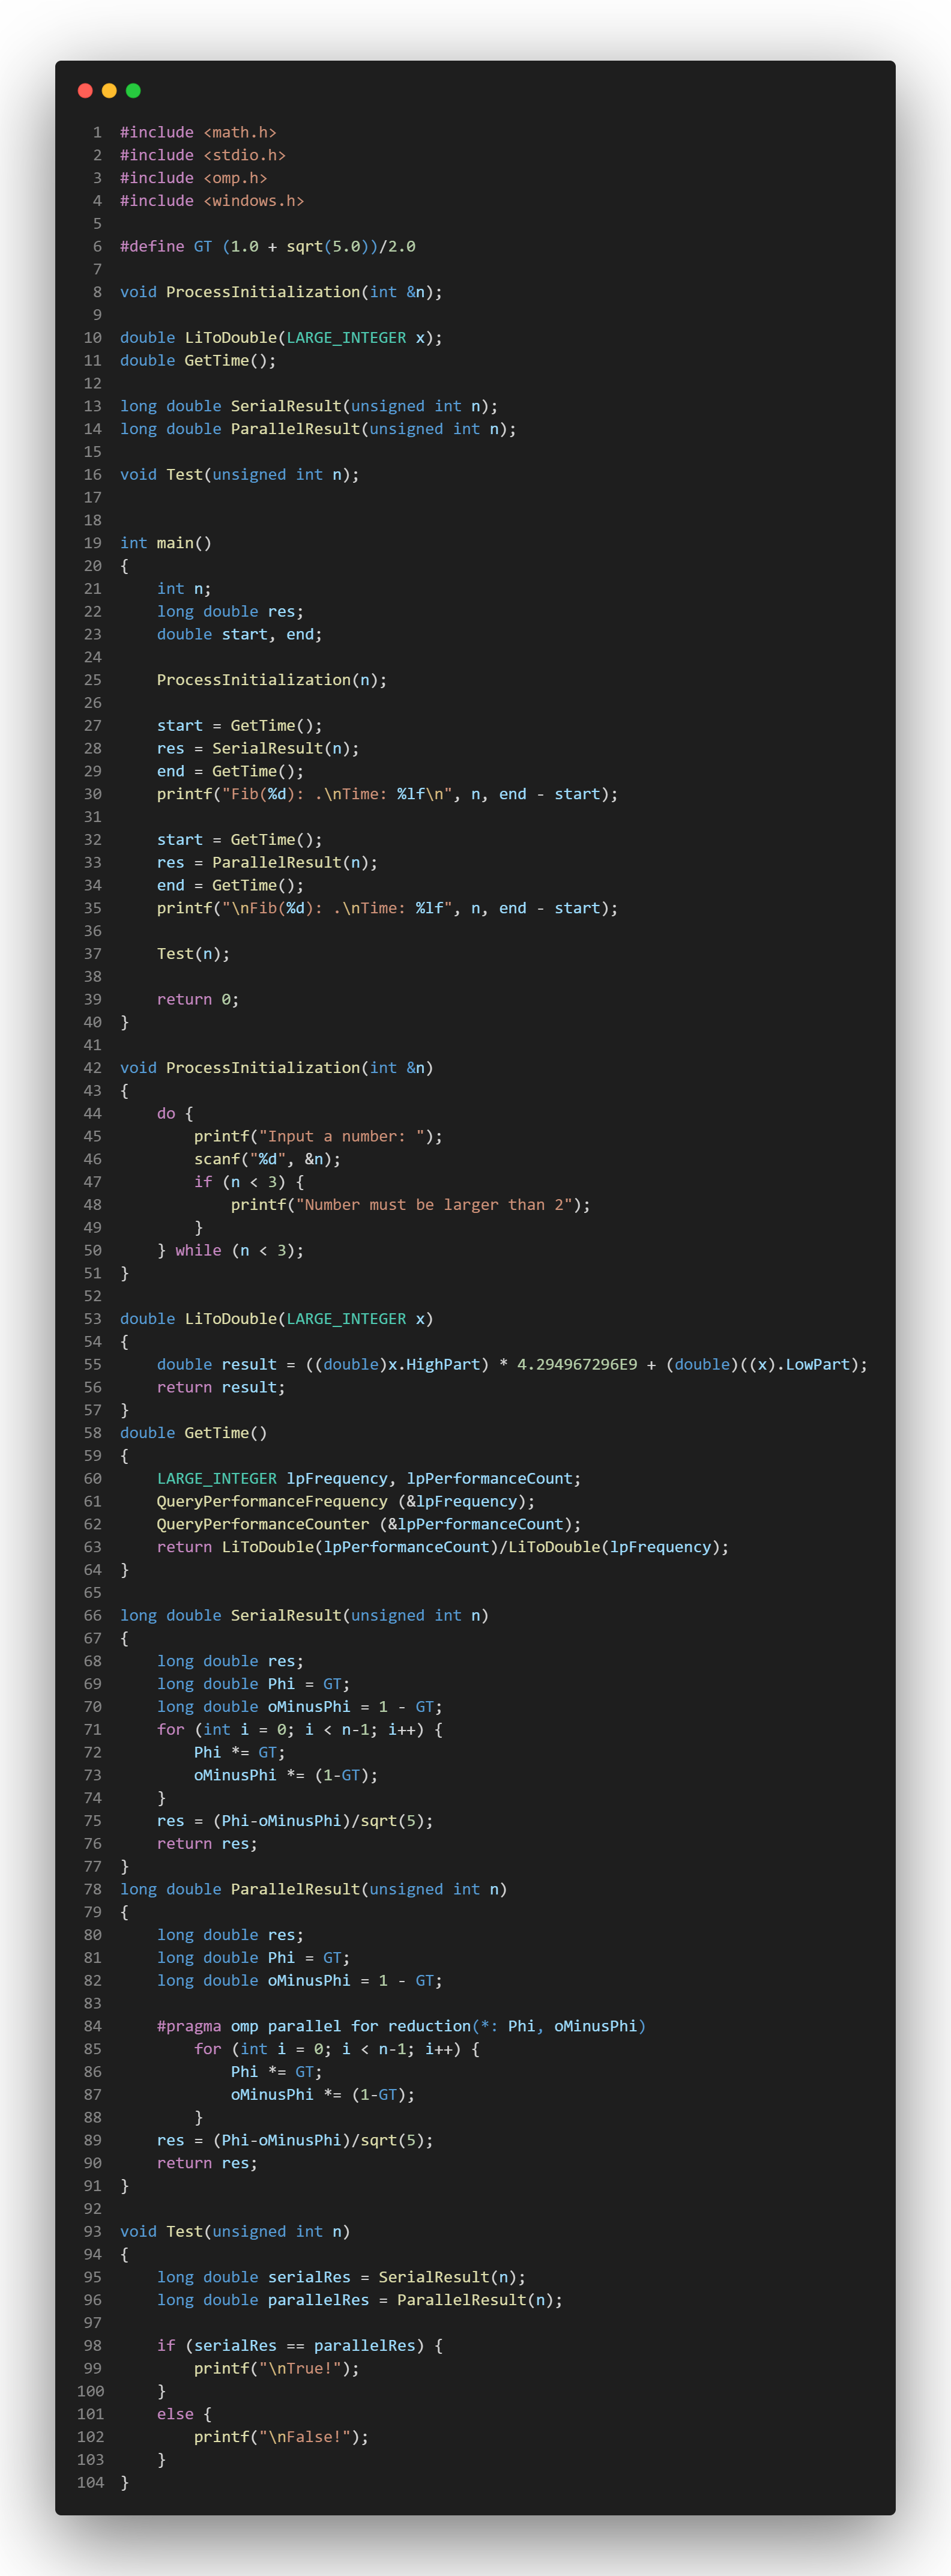
\includegraphics[trim=0in 0in 0in 49.75in, clip, scale=0.25]{./Photos/Fibonacci/Parallel.PNG}
\end{center}
\section{Đánh giá}
\begin{center}
	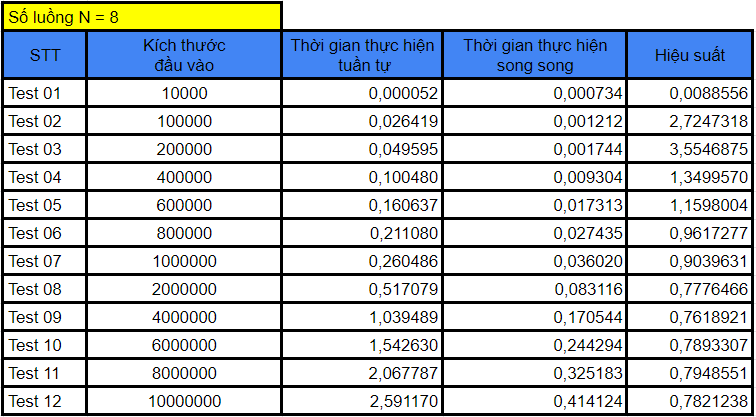
\includegraphics[scale=0.9]{./Photos/Fibonacci/Benchmark.PNG}
\end{center}


\chapter{Tính số PI}
\section{Thuật toán tuần tự}
\begin{center}
	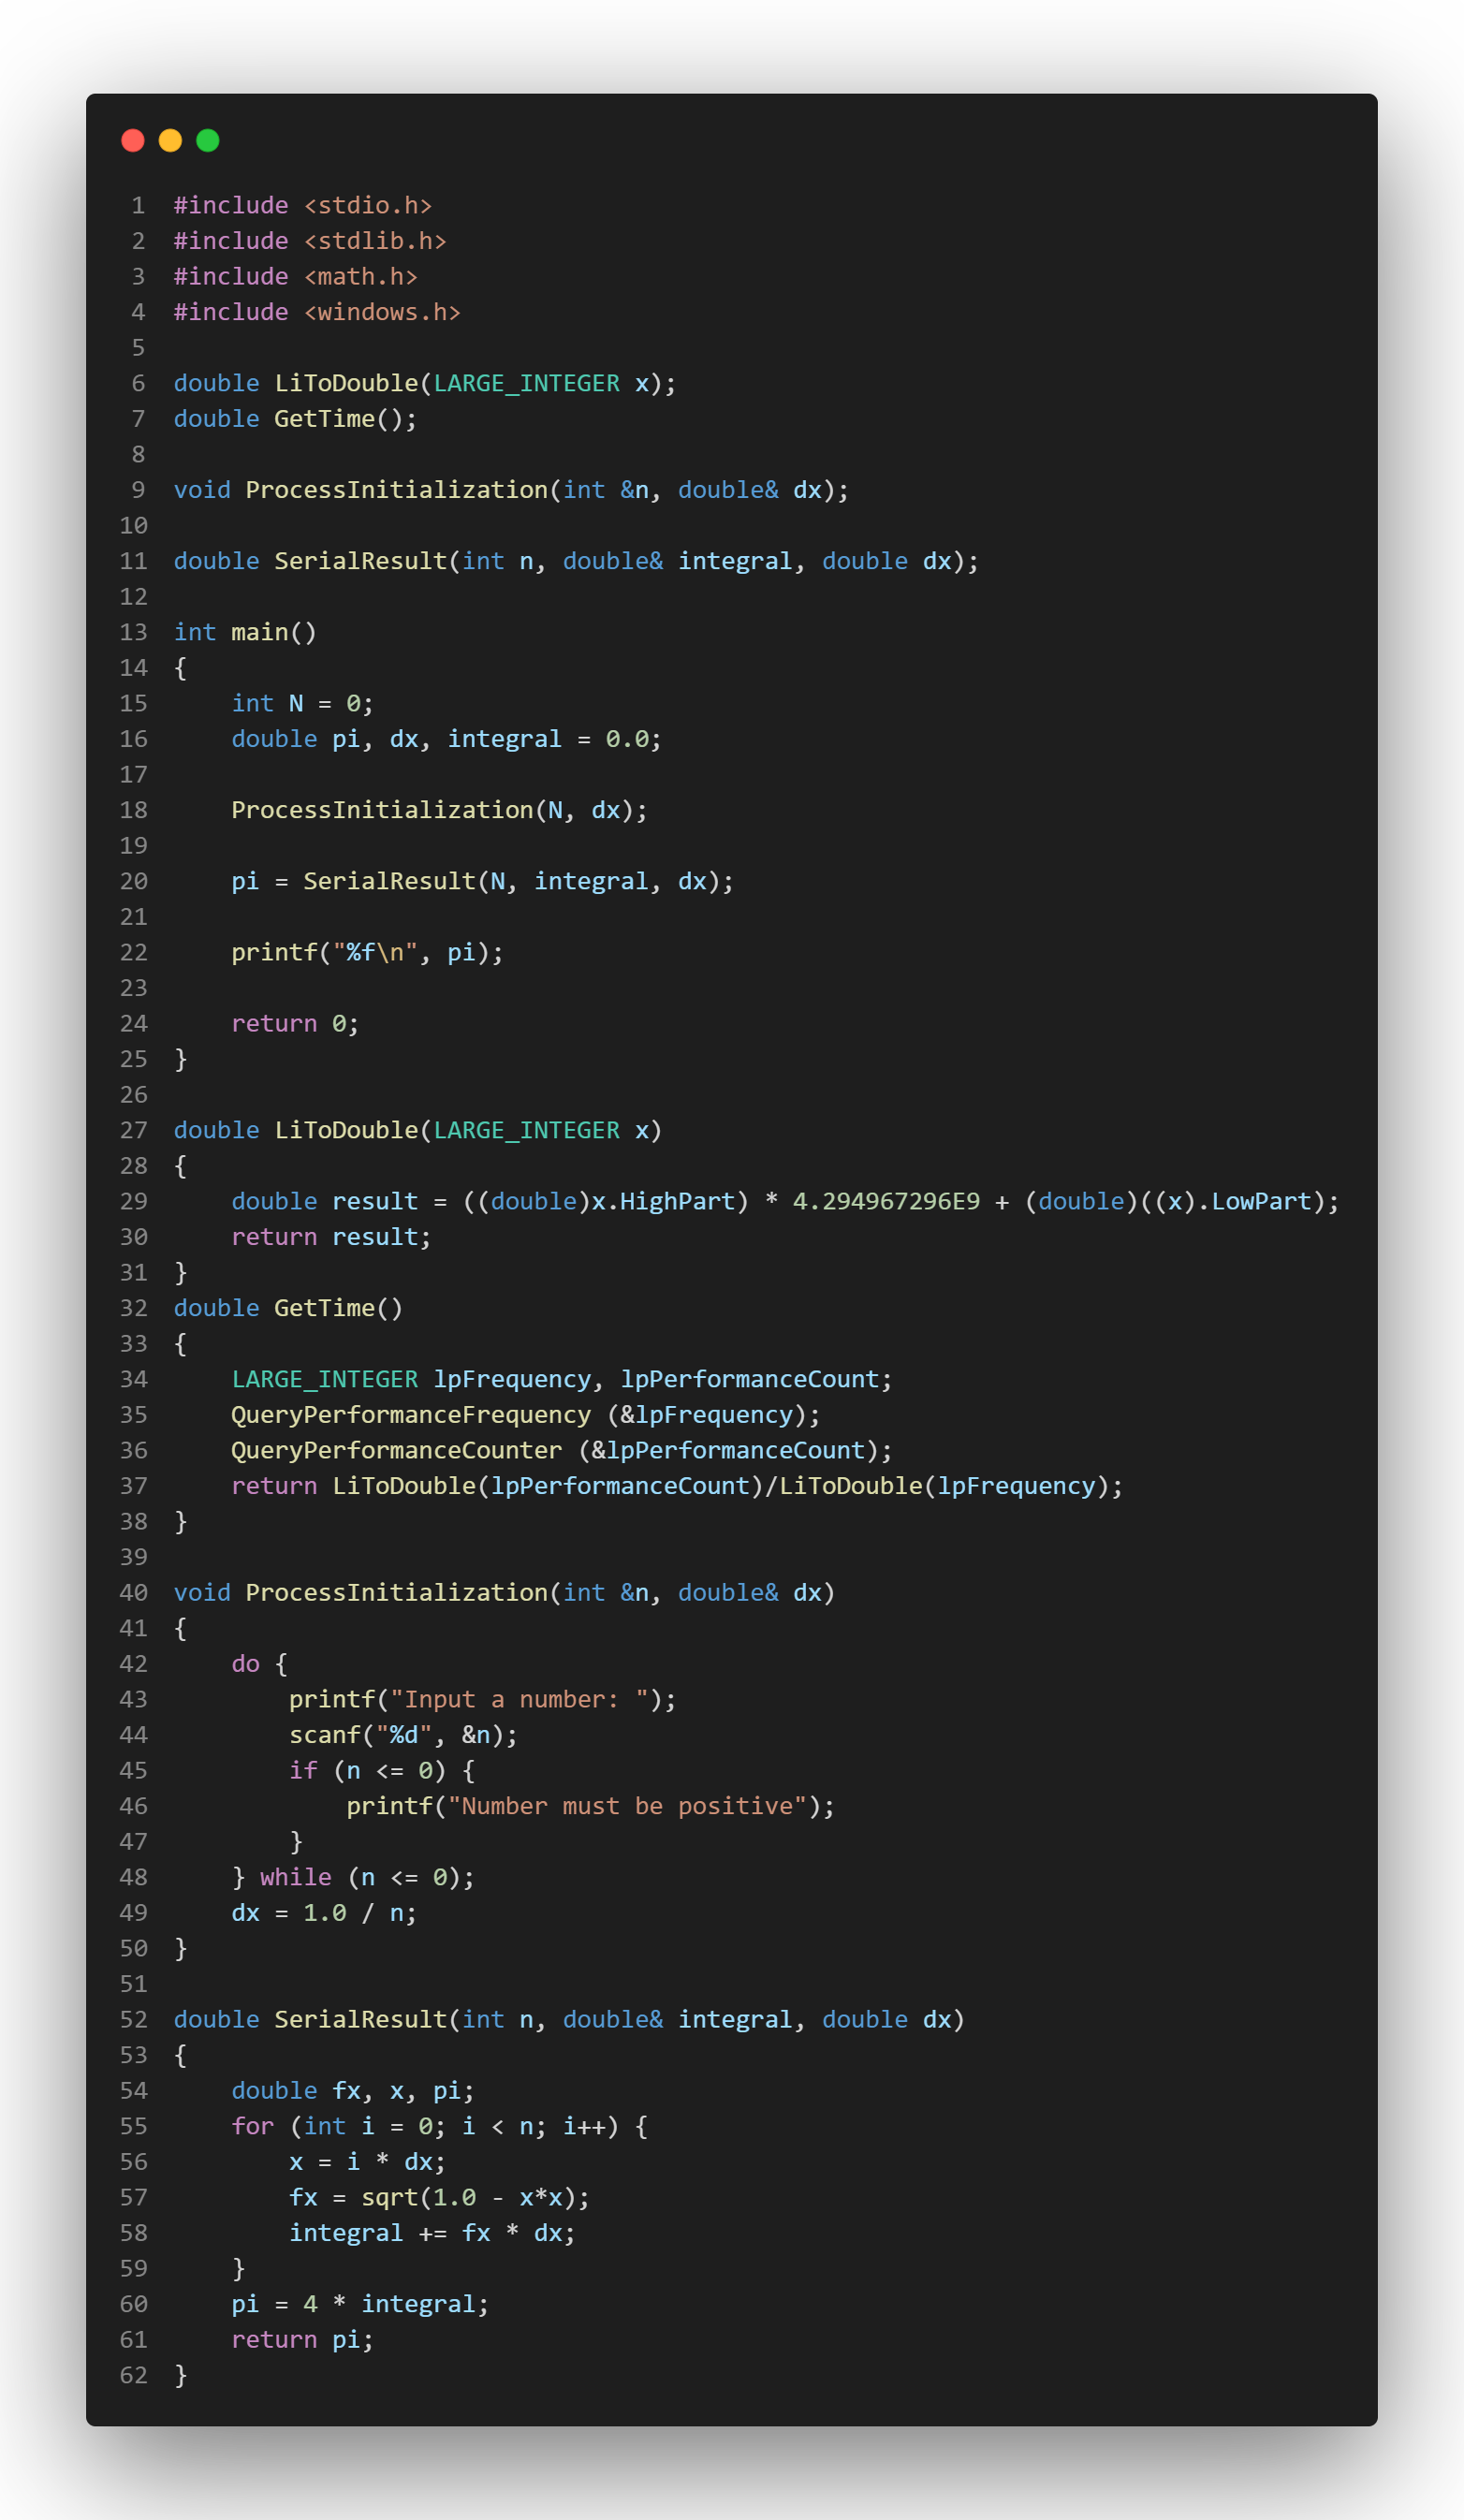
\includegraphics[trim=0in 13in 0in 0in, clip, scale=0.25]{./Photos/PI/serial.PNG}
\clearpage
	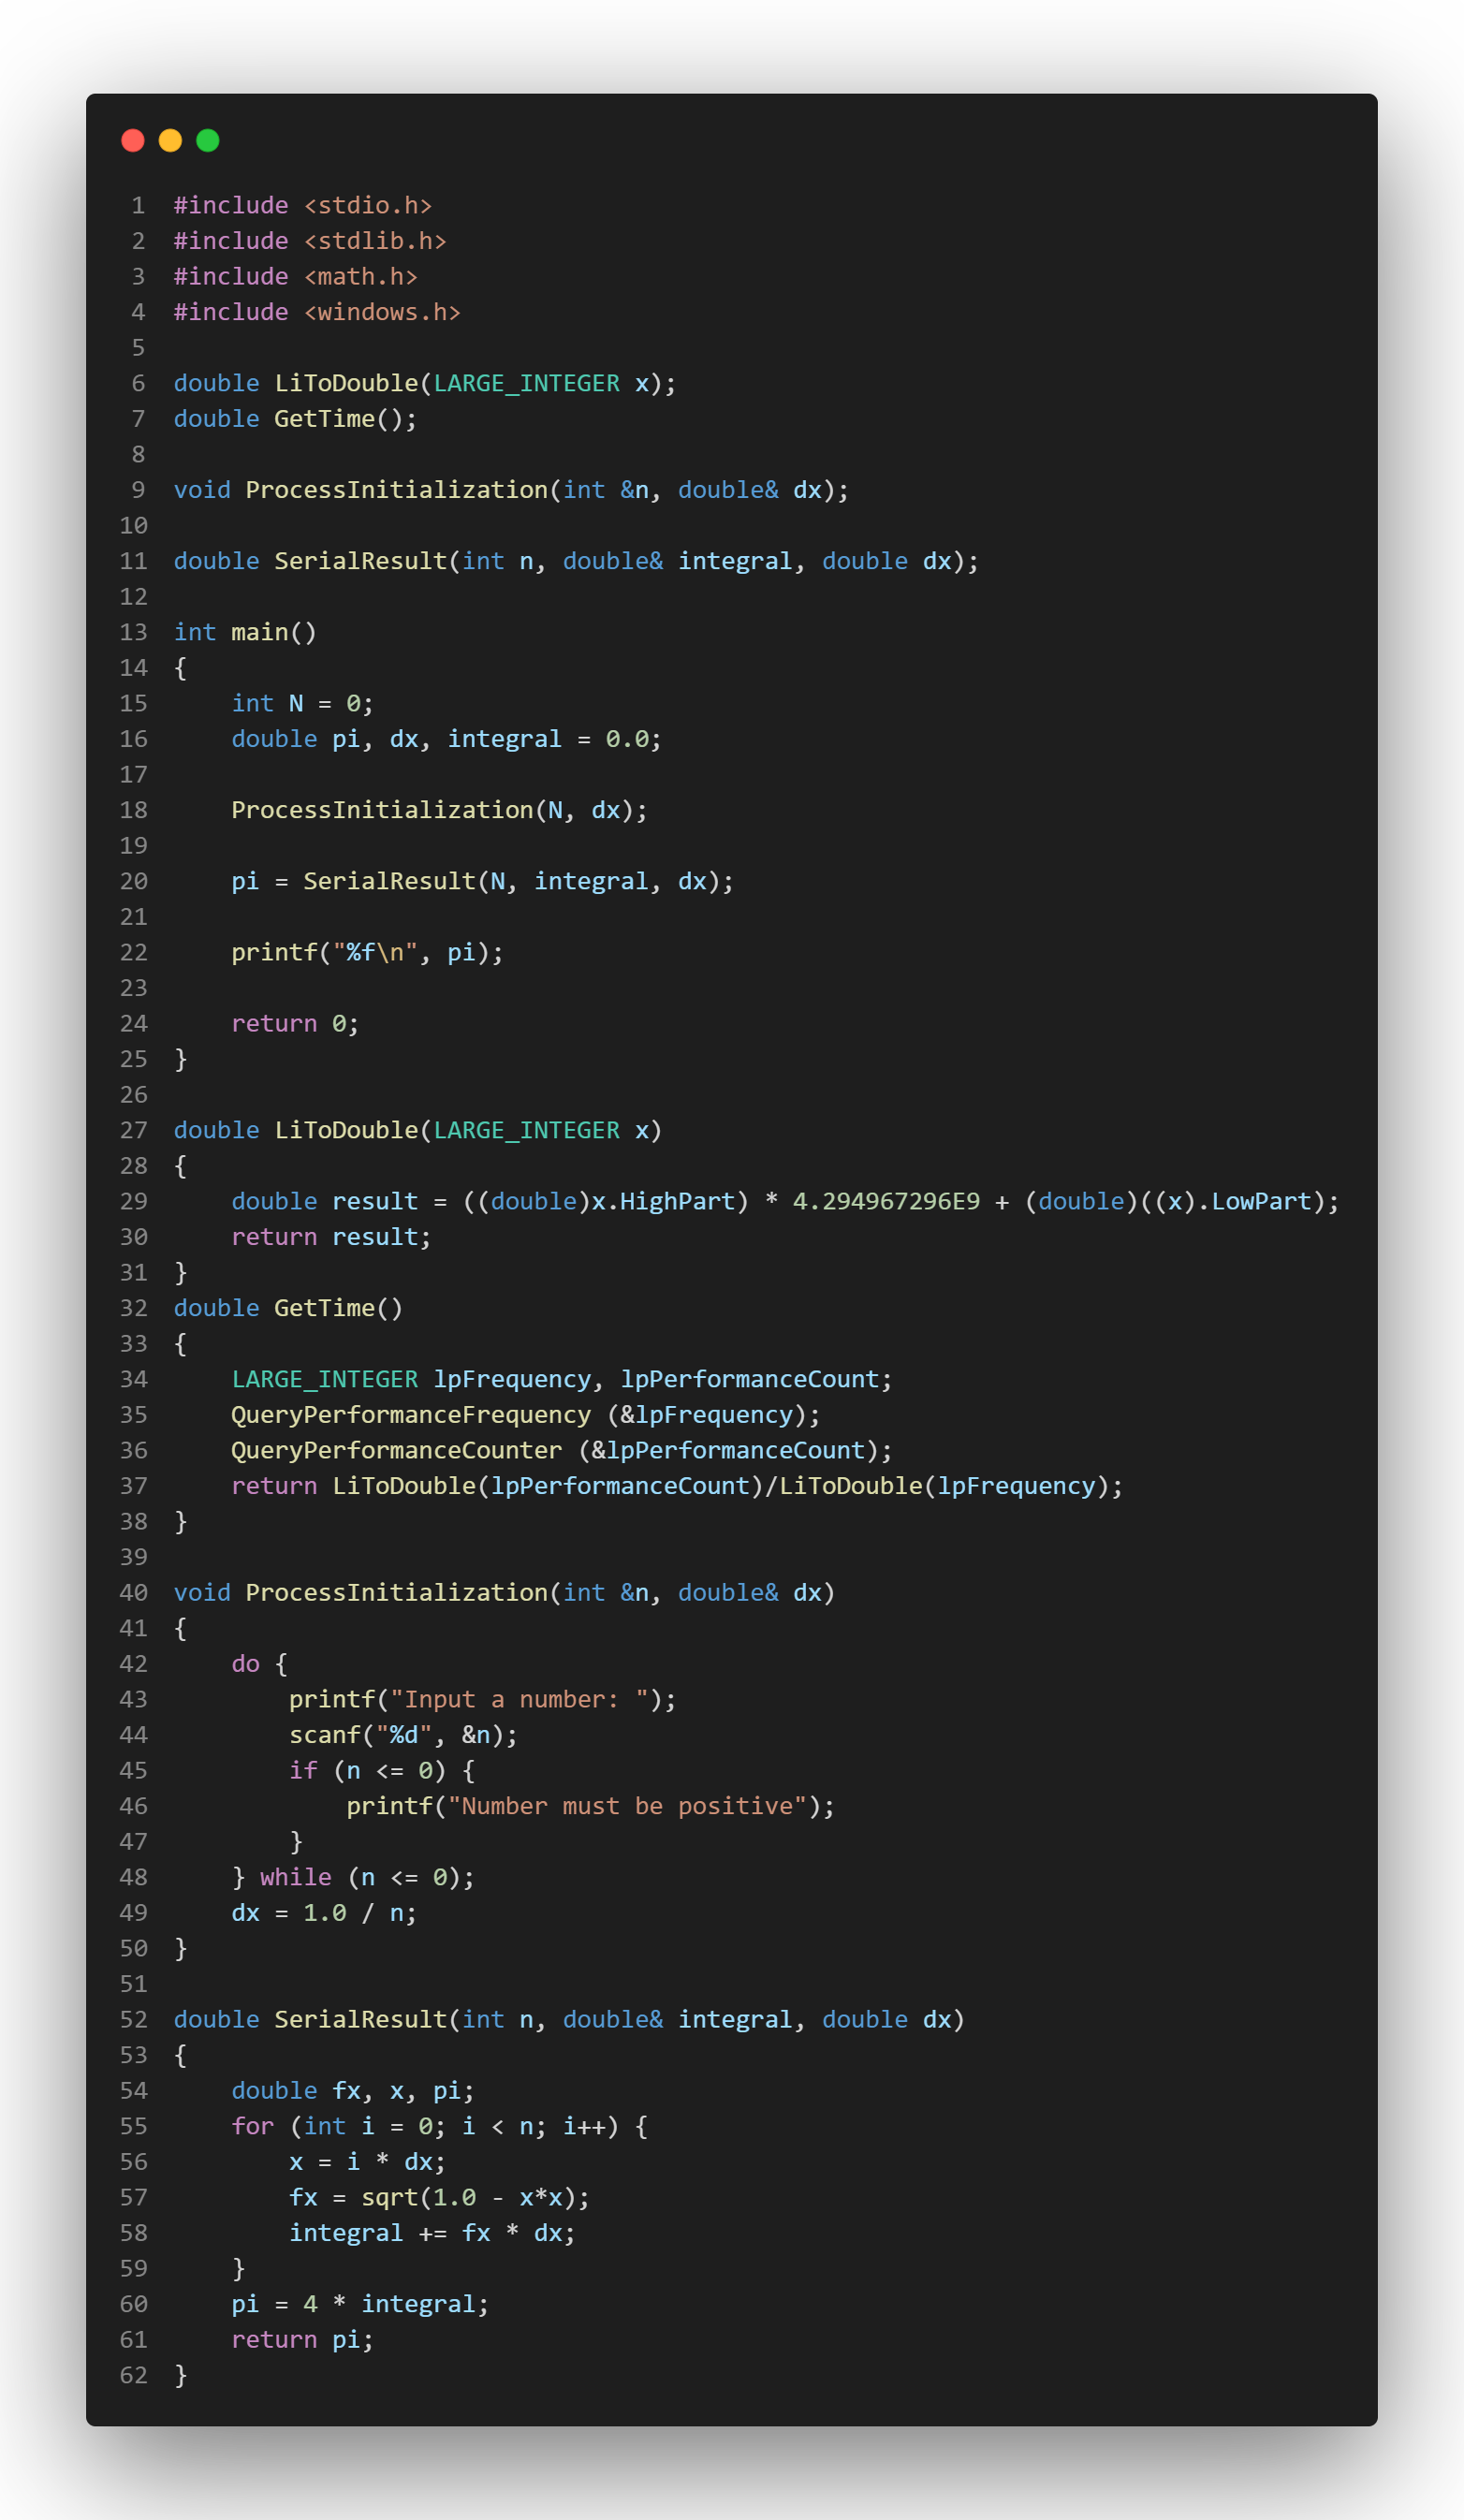
\includegraphics[trim=0in 0in 0in 24.5in, clip, scale=0.25]{./Photos/PI/serial.PNG}
\end{center}
\section{Thuật toán song song}
\begin{center}
	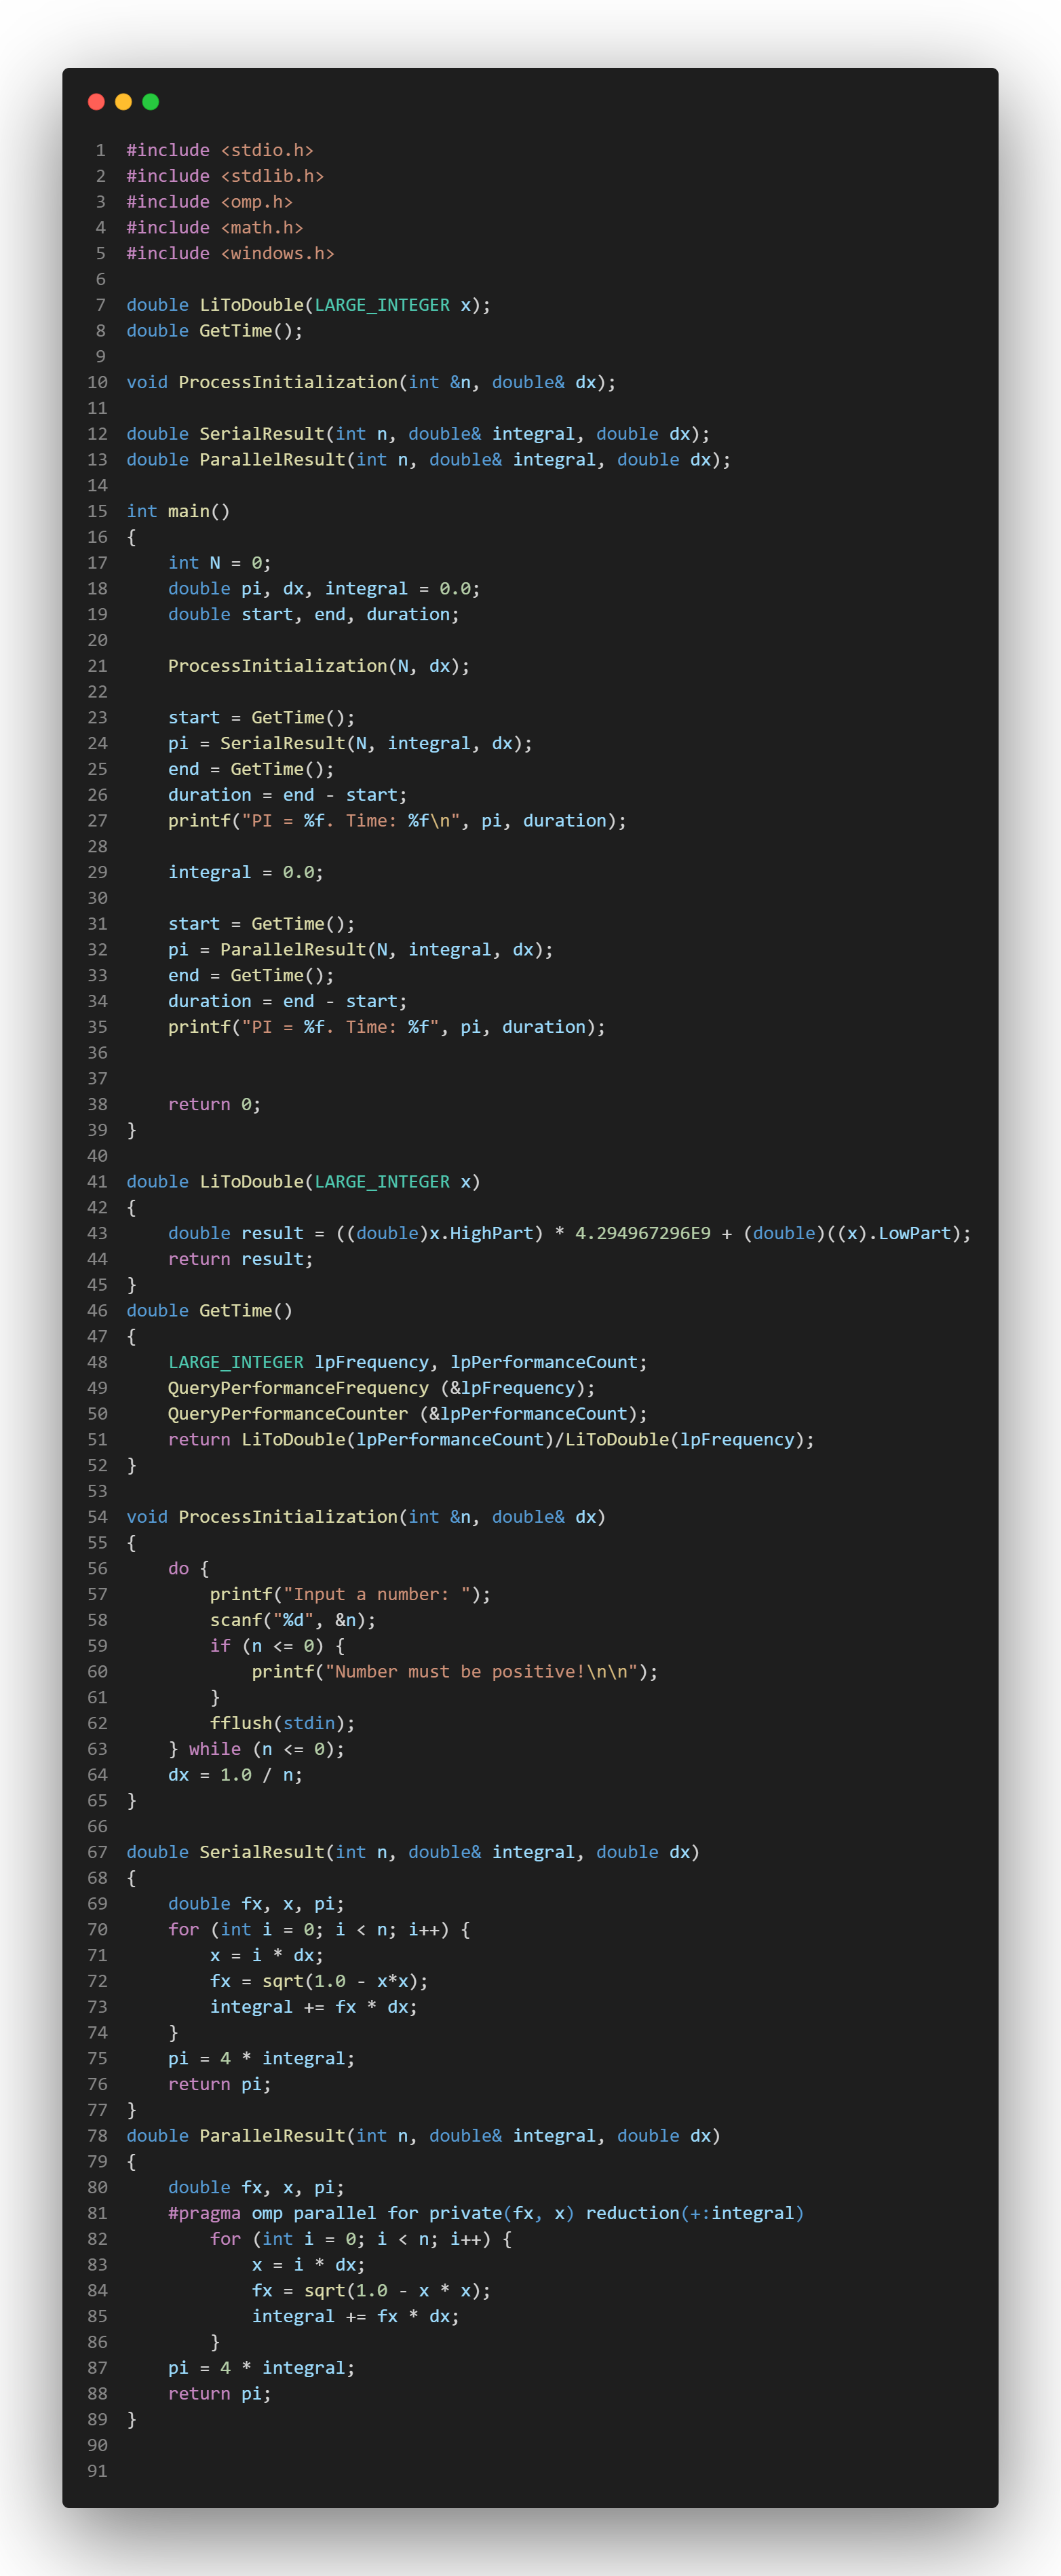
\includegraphics[trim=0in 33in 0in 0in, clip, scale=0.25]{./Photos/PI/parallel.PNG}
\clearpage
	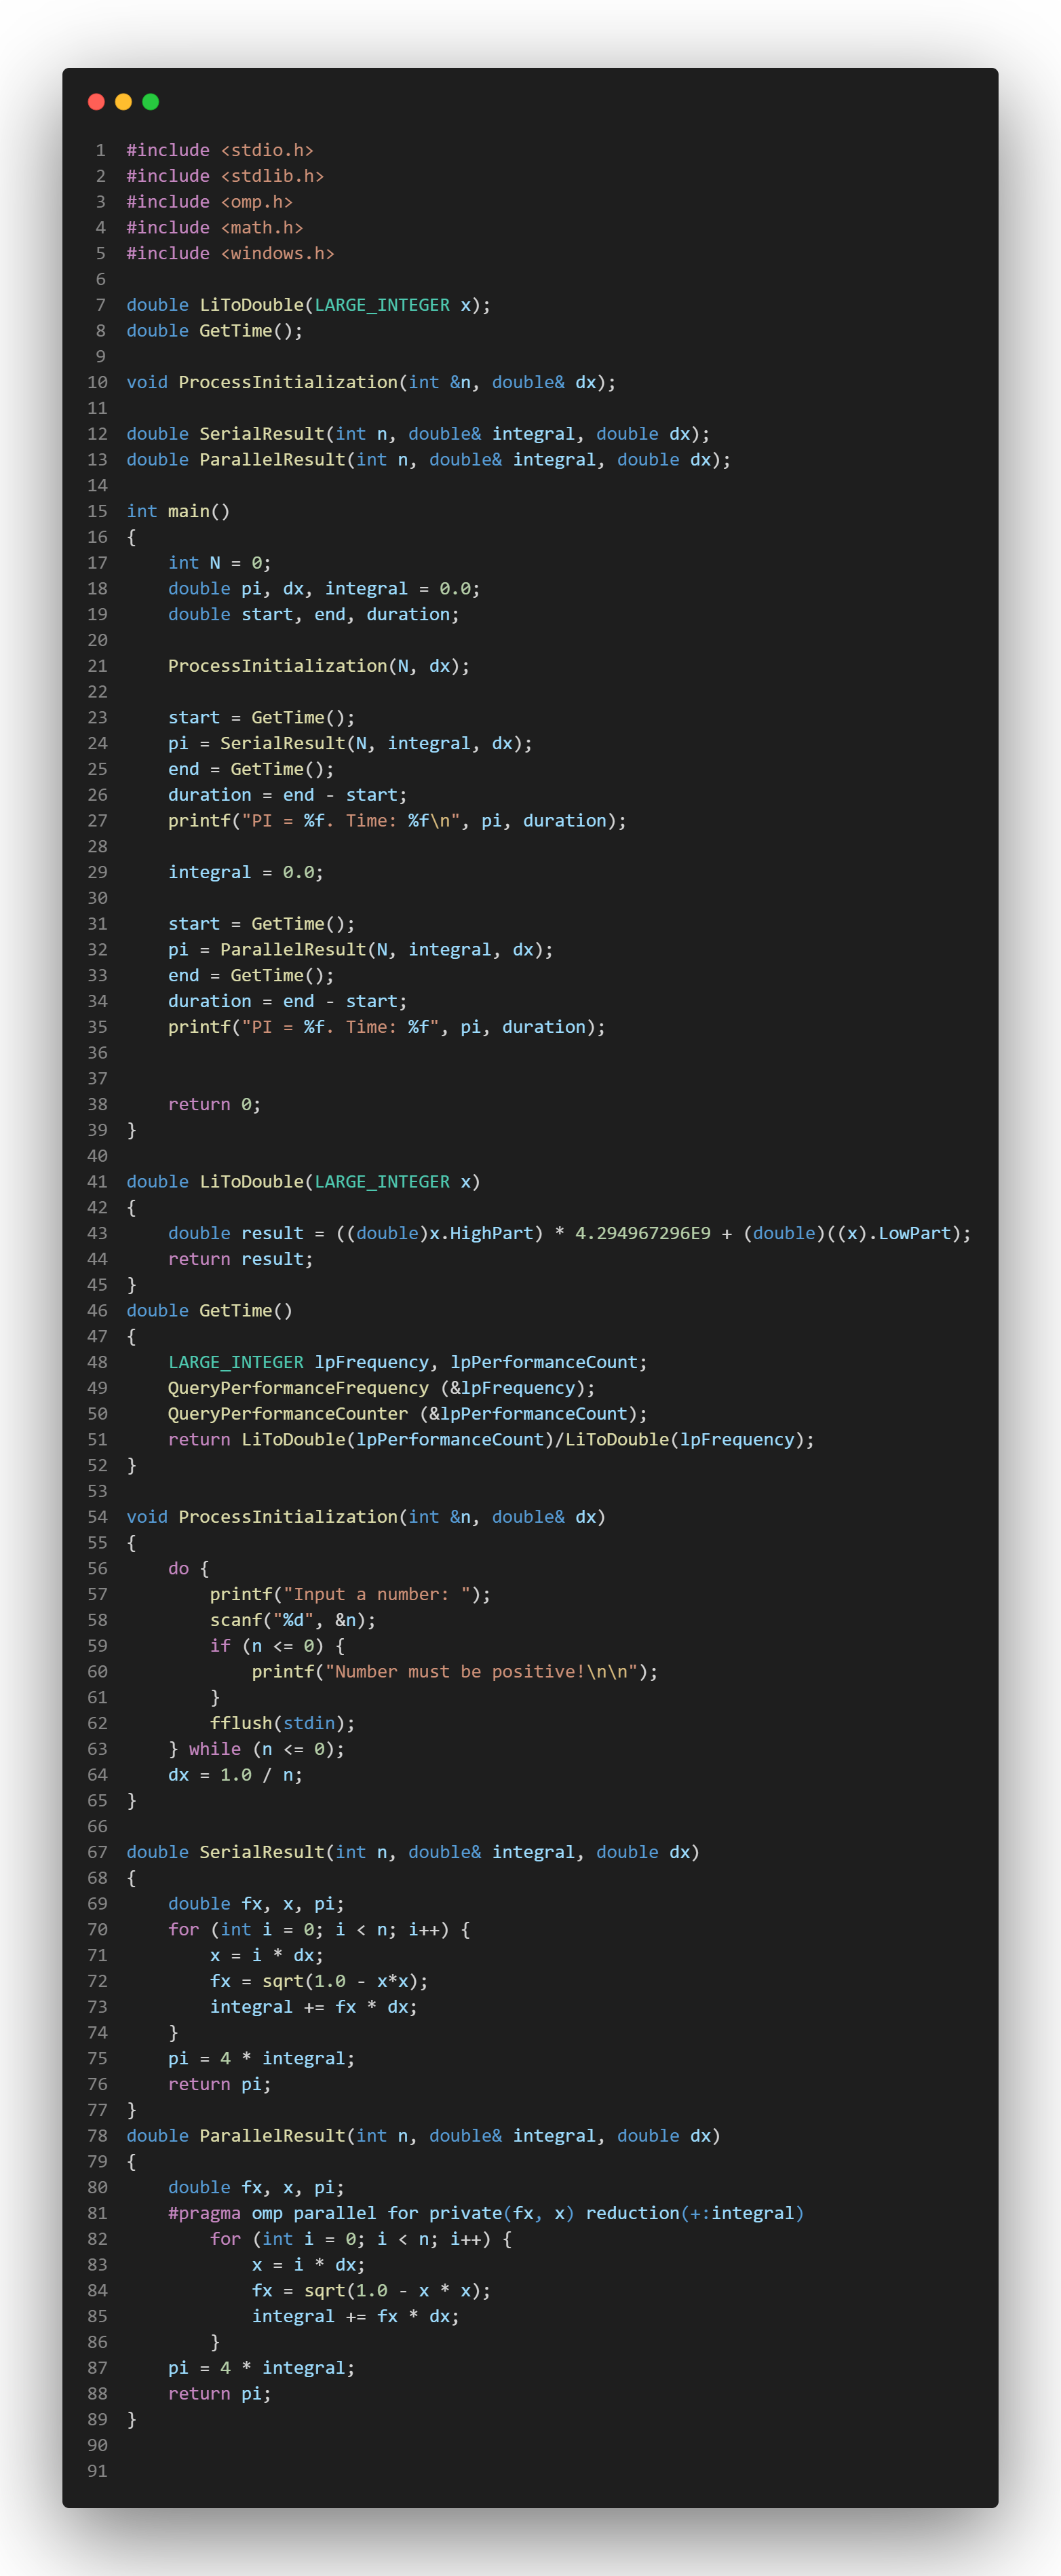
\includegraphics[trim=0in 0in 0in 19.75in, clip, scale=0.25]{./Photos/PI/parallel.PNG}
\end{center}
\section{Đánh giá}
\subsection{Trên Windows}
\begin{center}
	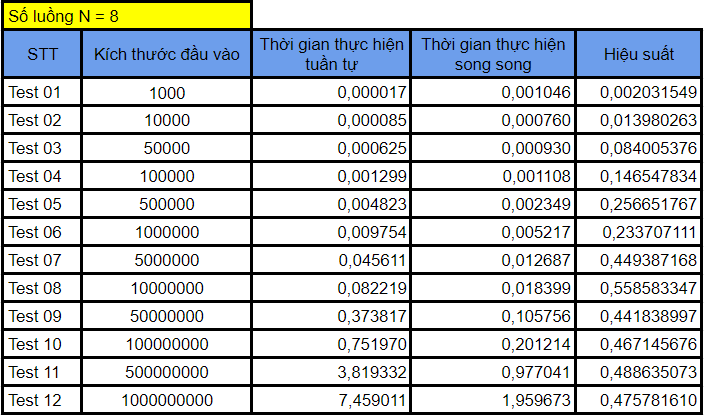
\includegraphics[scale=0.9]{./Photos/PI/BenchmarkOnWin.PNG}
\end{center}
\clearpage
\subsection{Trên Linux}
\begin{center}
	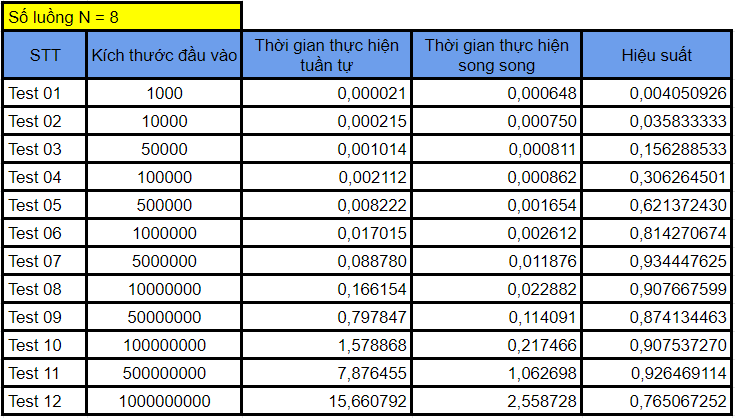
\includegraphics[scale=0.9]{./Photos/PI/BenchmarkOnLinux.PNG}
\end{center}


\chapter*{Kết luận}                         % Chương 3
\addcontentsline{toc}{chapter}{{\bf  Kết luận}\rm}
Do năng lực còn hạn chế cũng như thời gian có hạn, nên bài báo cáo còn xuất hiện nhiều sai sót, code còn sơ sài, một số bài toán kết quả chỉ mang tính chất minh họa do không tìm được cấu trúc dữ liệu phù hợp với bài toán (số lớn - Fibonacci, số lượng số sau dấu phẩy - PI). Ở phần đánh giá trên Linux, em sử dụng hệ điều hành ubuntu trên máy ảo nên kết quả đánh giá có thể không được chính xác khi so sánh với những máy thật sự chạy trên Linux. \\
Rất mong nhận được những lời nhận xét của thầy cũng như những người đọc được bài báo cáo này.


\begin{thebibliography}{99}               % Tài liệu tham khảo   
\addcontentsline{toc}{chapter}{{\bf  Tài liệu tham khảo}\rm} 

\bibitem{B} Bulić Patricio, Robič Borut, Slivnik Boštjan, Trobec Roman, {\it Introduction to Parallel Computing From Algorithms to Programming on State-of-the-Art Platforms}, 2018.
\bibitem{Tim} Tim Mattson, {\it Introduction to OpenMP}, Youtube.
\bibitem{Web} https://hpc.llnl.gov/training/tutorials.
\bibitem{Web} https://create.stephan-brumme.com/eratosthenes.
% Chú thích: mỗi tài liệu là một bibitem.

\end{thebibliography}


\end{document}

%Một số chú ý:
%-Sau phần \end{document} thì văn bản không còn hiển thị.
%-Các siêu liên kết (tên PT, định lí... được tham chiếu) thường có ô vuông đỏ bao quanh. Các bạn yên tâm, khi in ra sẽ ko xuất hiện cái ô vuông đó!